\pdfoutput=1
%% Author: PGL  Porta Mana
%% Created: 2015-05-01T20:53:34+0200
%% Last-Updated: 2019-07-21T17:05:52+0200
%%%%%%%%%%%%%%%%%%%%%%%%%%%%%%%%%%%%%%%%%%%%%%%%%%%%%%%%%%%%%%%%%%%%%%%%%%%%
\newif\ifarxiv
\arxivfalse
\ifarxiv\pdfmapfile{+classico.map}\fi
\newif\ifafour
\afourfalse% true = A4, false = A5
\newif\iftypodisclaim % typographical disclaim on the side
\typodisclaimtrue
\newcommand*{\memfontfamily}{zplx}
\newcommand*{\memfontpack}{newpxtext}
\documentclass[\ifafour a4paper,12pt,\else a5paper,10pt,\fi%extrafontsizes,%
onecolumn,oneside,article,%french,italian,german,swedish,latin,
british%
]{memoir}
\newcommand*{\updated}{\today}
\newcommand*{\firstdraft}{4 November 2015}
\newcommand*{\firstpublished}{***}
\newcommand*{\propertitle}{Maximum-entropy distributions for a 
  neuronal network\\ from subnetwork data%\\{\large ***}%
}
\newcommand*{\pdftitle}{\propertitle}
\newcommand*{\headtitle}{Maximum-entropy from sample data}
\newcommand*{\pdfauthor}{P.G.L.  Porta Mana, Y. Roudi, V. Rostami, E. Torre}
\newcommand*{\headauthor}{Porta Mana \etal}
\newcommand*{\reporthead}{}% Report number

%%%%%%%%%%%%%%%%%%%%%%%%%%%%%%%%%%%%%%%%%%%%%%%%%%%%%%%%%%%%%%%%%%%%%%%%%%%%
%%% Calls to packages (uncomment as needed)
%%%%%%%%%%%%%%%%%%%%%%%%%%%%%%%%%%%%%%%%%%%%%%%%%%%%%%%%%%%%%%%%%%%%%%%%%%%%

%\usepackage{pifont}

%\usepackage{fontawesome}

\usepackage[T1]{fontenc} 
\input{glyphtounicode} \pdfgentounicode=1

\usepackage[utf8]{inputenx}

%\usepackage{newunicodechar}
% \newunicodechar{Ĕ}{\u{E}}
% \newunicodechar{ĕ}{\u{e}}
% \newunicodechar{Ĭ}{\u{I}}
% \newunicodechar{ĭ}{\u{\i}}
% \newunicodechar{Ŏ}{\u{O}}
% \newunicodechar{ŏ}{\u{o}}
% \newunicodechar{Ŭ}{\u{U}}
% \newunicodechar{ŭ}{\u{u}}
% \newunicodechar{Ā}{\=A}
% \newunicodechar{ā}{\=a}
% \newunicodechar{Ē}{\=E}
% \newunicodechar{ē}{\=e}
% \newunicodechar{Ī}{\=I}
% \newunicodechar{ī}{\={\i}}
% \newunicodechar{Ō}{\=O}
% \newunicodechar{ō}{\=o}
% \newunicodechar{Ū}{\=U}
% \newunicodechar{ū}{\=u}
% \newunicodechar{Ȳ}{\=Y}
% \newunicodechar{ȳ}{\=y}

\newcommand*{\bmmax}{0} % reduce number of bold fonts, before font packages
\newcommand*{\hmmax}{0} % reduce number of heavy fonts, before font packages

\usepackage{textcomp}

%\usepackage[normalem]{ulem}% package for underlining
% \makeatletter
% \def\ssout{\bgroup \ULdepth=-.35ex%\UL@setULdepth
%  \markoverwith{\lower\ULdepth\hbox
%    {\kern-.03em\vbox{\hrule width.2em\kern1.2\p@\hrule}\kern-.03em}}%
%  \ULon}
% \makeatother

\usepackage{amsmath}

\usepackage{mathtools}
\addtolength{\jot}{\jot} % increase spacing in multiline formulae
\setlength{\multlinegap}{0pt}

%\usepackage{empheq}% automatically calls amsmath and mathtools
%\newcommand*{\widefbox}[1]{\fbox{\hspace{1em}#1\hspace{1em}}}

%\usepackage{fancybox}

%\usepackage{framed}

% \usepackage[misc]{ifsym} % for dice
% \newcommand*{\diceone}{{\scriptsize\Cube{1}}}

\usepackage{amssymb}

\usepackage{amsxtra}

\usepackage[main=british,french,italian,german,swedish,latin,esperanto]{babel}\selectlanguage{british}
\newcommand*{\langfrench}{\foreignlanguage{french}}
\newcommand*{\langgerman}{\foreignlanguage{german}}
\newcommand*{\langitalian}{\foreignlanguage{italian}}
\newcommand*{\langswedish}{\foreignlanguage{swedish}}
\newcommand*{\langlatin}{\foreignlanguage{latin}}
\newcommand*{\langnohyph}{\foreignlanguage{nohyphenation}}

\usepackage[autostyle=false,autopunct=false,english=british]{csquotes}
\setquotestyle{british}

\usepackage{amsthm}
\newcommand*{\QED}{\textsc{q.e.d.}}
\renewcommand*{\qedsymbol}{\QED}
\theoremstyle{remark}
\newtheorem{note}{Note}
\newtheorem*{remark}{Note}
\newtheoremstyle{innote}{\parsep}{\parsep}{\footnotesize}{}{}{}{0pt}{}
\theoremstyle{innote}
\newtheorem*{innote}{}

\usepackage[shortlabels,inline]{enumitem}
\SetEnumitemKey{para}{itemindent=\parindent,leftmargin=0pt,listparindent=\parindent,parsep=0pt,itemsep=\topsep}
% \begin{asparaenum} = \begin{enumerate}[para]
% \begin{inparaenum} = \begin{enumerate*}
\setlist[enumerate,2]{label=\alph*.}
\setlist[enumerate]{label=\arabic*.,leftmargin=1.5\parindent}
\setlist[itemize]{leftmargin=1.5\parindent}
\setlist[description]{leftmargin=1.5\parindent}
% old alternative:
% \setlist[enumerate,2]{label=\alph*.}
% \setlist[enumerate]{leftmargin=\parindent}
% \setlist[itemize]{leftmargin=\parindent}
% \setlist[description]{leftmargin=\parindent}

\usepackage[babel,theoremfont,largesc]{newpxtext}

\usepackage[bigdelims,nosymbolsc%,smallerops % probably arXiv doesn't have it
]{newpxmath}
\linespread{1.083}%\useosf
%% smaller operators for old version of newpxmath
\makeatletter
\def\re@DeclareMathSymbol#1#2#3#4{%
    \let#1=\undefined
    \DeclareMathSymbol{#1}{#2}{#3}{#4}}
%\re@DeclareMathSymbol{\bigsqcupop}{\mathop}{largesymbols}{"46}
%\re@DeclareMathSymbol{\bigodotop}{\mathop}{largesymbols}{"4A}
\re@DeclareMathSymbol{\bigoplusop}{\mathop}{largesymbols}{"4C}
\re@DeclareMathSymbol{\bigotimesop}{\mathop}{largesymbols}{"4E}
\re@DeclareMathSymbol{\sumop}{\mathop}{largesymbols}{"50}
\re@DeclareMathSymbol{\prodop}{\mathop}{largesymbols}{"51}
\re@DeclareMathSymbol{\bigcupop}{\mathop}{largesymbols}{"53}
\re@DeclareMathSymbol{\bigcapop}{\mathop}{largesymbols}{"54}
%\re@DeclareMathSymbol{\biguplusop}{\mathop}{largesymbols}{"55}
\re@DeclareMathSymbol{\bigwedgeop}{\mathop}{largesymbols}{"56}
\re@DeclareMathSymbol{\bigveeop}{\mathop}{largesymbols}{"57}
%\re@DeclareMathSymbol{\bigcupdotop}{\mathop}{largesymbols}{"DF}
%\re@DeclareMathSymbol{\bigcapplusop}{\mathop}{largesymbolsPXA}{"00}
%\re@DeclareMathSymbol{\bigsqcupplusop}{\mathop}{largesymbolsPXA}{"02}
%\re@DeclareMathSymbol{\bigsqcapplusop}{\mathop}{largesymbolsPXA}{"04}
%\re@DeclareMathSymbol{\bigsqcapop}{\mathop}{largesymbolsPXA}{"06}
\re@DeclareMathSymbol{\bigtimesop}{\mathop}{largesymbolsPXA}{"10}
%\re@DeclareMathSymbol{\coprodop}{\mathop}{largesymbols}{"60}
%\re@DeclareMathSymbol{\varprod}{\mathop}{largesymbolsPXA}{16}
\makeatother
%%
%% With euler font cursive for Greek letters - the [1] means 100% scaling
\DeclareFontFamily{U}{egreek}{\skewchar\font'177}%
\DeclareFontShape{U}{egreek}{m}{n}{<-6>s*[1]eurm5 <6-8>s*[1]eurm7 <8->s*[1]eurm10}{}%
\DeclareFontShape{U}{egreek}{m}{it}{<->s*[1]eurmo10}{}%
\DeclareFontShape{U}{egreek}{b}{n}{<-6>s*[1]eurb5 <6-8>s*[1]eurb7 <8->s*[1]eurb10}{}%
\DeclareFontShape{U}{egreek}{b}{it}{<->s*[1]eurbo10}{}%
\DeclareSymbolFont{egreeki}{U}{egreek}{m}{it}%
\SetSymbolFont{egreeki}{bold}{U}{egreek}{b}{it}% from the amsfonts package
\DeclareSymbolFont{egreekr}{U}{egreek}{m}{n}%
\SetSymbolFont{egreekr}{bold}{U}{egreek}{b}{n}% from the amsfonts package
% Take also \sum, \prod, \coprod symbols from Euler fonts
\DeclareFontFamily{U}{egreekx}{\skewchar\font'177}
\DeclareFontShape{U}{egreekx}{m}{n}{%
       <-7.5>s*[0.9]euex7%
    <7.5-8.5>s*[0.9]euex8%
    <8.5-9.5>s*[0.9]euex9%
    <9.5->s*[0.9]euex10%
}{}
\DeclareSymbolFont{egreekx}{U}{egreekx}{m}{n}
\DeclareMathSymbol{\sumop}{\mathop}{egreekx}{"50}
\DeclareMathSymbol{\prodop}{\mathop}{egreekx}{"51}
\DeclareMathSymbol{\coprodop}{\mathop}{egreekx}{"60}
\makeatletter
\def\sum{\DOTSI\sumop\slimits@}
\def\prod{\DOTSI\prodop\slimits@}
\def\coprod{\DOTSI\coprodop\slimits@}
\makeatother
% Greek letters not usually given in LaTeX.
\DeclareMathSymbol{\varpartial}{\mathalpha}{egreeki}{"40}
\DeclareMathSymbol{\partialup}{\mathalpha}{egreekr}{"40}
\DeclareMathSymbol{\alpha}{\mathalpha}{egreeki}{"0B}
\DeclareMathSymbol{\beta}{\mathalpha}{egreeki}{"0C}
\DeclareMathSymbol{\gamma}{\mathalpha}{egreeki}{"0D}
\DeclareMathSymbol{\delta}{\mathalpha}{egreeki}{"0E}
\DeclareMathSymbol{\epsilon}{\mathalpha}{egreeki}{"0F}
\DeclareMathSymbol{\zeta}{\mathalpha}{egreeki}{"10}
\DeclareMathSymbol{\eta}{\mathalpha}{egreeki}{"11}
\DeclareMathSymbol{\theta}{\mathalpha}{egreeki}{"12}
\DeclareMathSymbol{\iota}{\mathalpha}{egreeki}{"13}
\DeclareMathSymbol{\kappa}{\mathalpha}{egreeki}{"14}
\DeclareMathSymbol{\lambda}{\mathalpha}{egreeki}{"15}
\DeclareMathSymbol{\mu}{\mathalpha}{egreeki}{"16}
\DeclareMathSymbol{\nu}{\mathalpha}{egreeki}{"17}
\DeclareMathSymbol{\xi}{\mathalpha}{egreeki}{"18}
\DeclareMathSymbol{\omicron}{\mathalpha}{egreeki}{"6F}
\DeclareMathSymbol{\pi}{\mathalpha}{egreeki}{"19}
\DeclareMathSymbol{\rho}{\mathalpha}{egreeki}{"1A}
\DeclareMathSymbol{\sigma}{\mathalpha}{egreeki}{"1B}
 \DeclareMathSymbol{\tau}{\mathalpha}{egreeki}{"1C}
\DeclareMathSymbol{\upsilon}{\mathalpha}{egreeki}{"1D}
\DeclareMathSymbol{\phi}{\mathalpha}{egreeki}{"1E}
\DeclareMathSymbol{\chi}{\mathalpha}{egreeki}{"1F}
\DeclareMathSymbol{\psi}{\mathalpha}{egreeki}{"20}
\DeclareMathSymbol{\omega}{\mathalpha}{egreeki}{"21}
\DeclareMathSymbol{\varepsilon}{\mathalpha}{egreeki}{"22}
\DeclareMathSymbol{\vartheta}{\mathalpha}{egreeki}{"23}
\DeclareMathSymbol{\varpi}{\mathalpha}{egreeki}{"24}
\let\varrho\rho 
\let\varsigma\sigma
 \let\varkappa\kappa
\DeclareMathSymbol{\varphi}{\mathalpha}{egreeki}{"27}
%
\DeclareMathSymbol{\varAlpha}{\mathalpha}{egreeki}{"41}
\DeclareMathSymbol{\varBeta}{\mathalpha}{egreeki}{"42}
\DeclareMathSymbol{\varGamma}{\mathalpha}{egreeki}{"00}
\DeclareMathSymbol{\varDelta}{\mathalpha}{egreeki}{"01}
\DeclareMathSymbol{\varEpsilon}{\mathalpha}{egreeki}{"45}
\DeclareMathSymbol{\varZeta}{\mathalpha}{egreeki}{"5A}
\DeclareMathSymbol{\varEta}{\mathalpha}{egreeki}{"48}
\DeclareMathSymbol{\varTheta}{\mathalpha}{egreeki}{"02}
 \DeclareMathSymbol{\varIota}{\mathalpha}{egreeki}{"49}
\DeclareMathSymbol{\varKappa}{\mathalpha}{egreeki}{"4B}
\DeclareMathSymbol{\varLambda}{\mathalpha}{egreeki}{"03}
\DeclareMathSymbol{\varMu}{\mathalpha}{egreeki}{"4D}
\DeclareMathSymbol{\varNu}{\mathalpha}{egreeki}{"4E}
\DeclareMathSymbol{\varXi}{\mathalpha}{egreeki}{"04}
\DeclareMathSymbol{\varOmicron}{\mathalpha}{egreeki}{"4F}
\DeclareMathSymbol{\varPi}{\mathalpha}{egreeki}{"05}
\DeclareMathSymbol{\varRho}{\mathalpha}{egreeki}{"50}
\DeclareMathSymbol{\varSigma}{\mathalpha}{egreeki}{"06}
\DeclareMathSymbol{\varTau}{\mathalpha}{egreeki}{"54}
\DeclareMathSymbol{\varUpsilon}{\mathalpha}{egreeki}{"07}
\DeclareMathSymbol{\varPhi}{\mathalpha}{egreeki}{"08}
\DeclareMathSymbol{\varChi}{\mathalpha}{egreeki}{"58}
\DeclareMathSymbol{\varPsi}{\mathalpha}{egreeki}{"09}
\DeclareMathSymbol{\varOmega}{\mathalpha}{egreeki}{"0A} 
%
\DeclareMathSymbol{\Alpha}{\mathalpha}{egreekr}{"41}
\DeclareMathSymbol{\Beta}{\mathalpha}{egreekr}{"42}
\DeclareMathSymbol{\Gamma}{\mathalpha}{egreekr}{"00}
\DeclareMathSymbol{\Delta}{\mathalpha}{egreekr}{"01}
\DeclareMathSymbol{\Epsilon}{\mathalpha}{egreekr}{"45}
\DeclareMathSymbol{\Zeta}{\mathalpha}{egreekr}{"5A}
\DeclareMathSymbol{\Eta}{\mathalpha}{egreekr}{"48}
\DeclareMathSymbol{\Theta}{\mathalpha}{egreekr}{"02}
\DeclareMathSymbol{\Iota}{\mathalpha}{egreekr}{"49}
\DeclareMathSymbol{\Kappa}{\mathalpha}{egreekr}{"4B}
\DeclareMathSymbol{\Lambda}{\mathalpha}{egreekr}{"03}
\DeclareMathSymbol{\Mu}{\mathalpha}{egreekr}{"4D}
\DeclareMathSymbol{\Nu}{\mathalpha}{egreekr}{"4E}
\DeclareMathSymbol{\Xi}{\mathalpha}{egreekr}{"04}
\DeclareMathSymbol{\Omicron}{\mathalpha}{egreekr}{"4F}
\DeclareMathSymbol{\Pi}{\mathalpha}{egreekr}{"05}
\DeclareMathSymbol{\Rho}{\mathalpha}{egreekr}{"50}
\DeclareMathSymbol{\Sigma}{\mathalpha}{egreekr}{"06}
\DeclareMathSymbol{\Tau}{\mathalpha}{egreekr}{"54}
\DeclareMathSymbol{\Upsilon}{\mathalpha}{egreekr}{"07}
\DeclareMathSymbol{\Phi}{\mathalpha}{egreekr}{"08}
\DeclareMathSymbol{\Chi}{\mathalpha}{egreekr}{"58}
\DeclareMathSymbol{\Psi}{\mathalpha}{egreekr}{"09}
\DeclareMathSymbol{\Omega}{\mathalpha}{egreekr}{"0A}
%
\DeclareMathSymbol{\alphaup}{\mathalpha}{egreekr}{"0B}
\DeclareMathSymbol{\betaup}{\mathalpha}{egreekr}{"0C}
\DeclareMathSymbol{\gammaup}{\mathalpha}{egreekr}{"0D}
 \DeclareMathSymbol{\deltaup}{\mathalpha}{egreekr}{"0E}
\DeclareMathSymbol{\epsilonup}{\mathalpha}{egreekr}{"0F}
\DeclareMathSymbol{\zetaup}{\mathalpha}{egreekr}{"10}
\DeclareMathSymbol{\etaup}{\mathalpha}{egreekr}{"11}
\DeclareMathSymbol{\thetaup}{\mathalpha}{egreekr}{"12}
\DeclareMathSymbol{\iotaup}{\mathalpha}{egreekr}{"13}
\DeclareMathSymbol{\kappaup}{\mathalpha}{egreekr}{"14}
\DeclareMathSymbol{\lambdaup}{\mathalpha}{egreekr}{"15}
\DeclareMathSymbol{\muup}{\mathalpha}{egreekr}{"16}
\DeclareMathSymbol{\nuup}{\mathalpha}{egreekr}{"17}
\DeclareMathSymbol{\xiup}{\mathalpha}{egreekr}{"18}
\DeclareMathSymbol{\omicronup}{\mathalpha}{egreekr}{"6F}
  \DeclareMathSymbol{\piup}{\mathalpha}{egreekr}{"19}
\DeclareMathSymbol{\rhoup}{\mathalpha}{egreekr}{"1A}
\DeclareMathSymbol{\sigmaup}{\mathalpha}{egreekr}{"1B}
\DeclareMathSymbol{\tauup}{\mathalpha}{egreekr}{"1C}
\DeclareMathSymbol{\upsilonup}{\mathalpha}{egreekr}{"1D}
\DeclareMathSymbol{\phiup}{\mathalpha}{egreekr}{"1E}
\DeclareMathSymbol{\chiup}{\mathalpha}{egreekr}{"1F}
\DeclareMathSymbol{\psiup}{\mathalpha}{egreekr}{"20}
\DeclareMathSymbol{\omegaup}{\mathalpha}{egreekr}{"21}
\DeclareMathSymbol{\varepsilonup}{\mathalpha}{egreekr}{"22}
\DeclareMathSymbol{\varthetaup}{\mathalpha}{egreekr}{"23}
\DeclareMathSymbol{\varpiup}{\mathalpha}{egreekr}{"24}
\let\varrhoup\rhoup 
\let\varsigmaup\sigmaup
\let\varkappaup\kappaup
\DeclareMathSymbol{\varphiup}{\mathalpha}{egreekr}{"27}
% Greek letters not usually given in LaTeX.

%\usepackage%[scaled=0.9]%
%{classico}%  Optima as sans-serif font
\renewcommand\sfdefault{uop}
\DeclareMathAlphabet{\mathsf}  {T1}{\sfdefault}{m}{sl}
\SetMathAlphabet{\mathsf}{bold}{T1}{\sfdefault}{b}{sl}
\newcommand*{\mathte}[1]{\textbf{\textit{\textsf{#1}}}}
% Upright sans-serif math alphabet
% \DeclareMathAlphabet{\mathsu}  {T1}{\sfdefault}{m}{n}
% \SetMathAlphabet{\mathsu}{bold}{T1}{\sfdefault}{b}{n}

% DejaVu Mono as typewriter text
\usepackage[scaled=0.84]{DejaVuSansMono}

\usepackage{mathdots}

\usepackage[usenames]{xcolor}
% Tol (2012) colour-blind-, print-, screen-friendly colours, alternative scheme; Munsell terminology
\definecolor{mypurpleblue}{RGB}{68,119,170}
\definecolor{myblue}{RGB}{102,204,238}
\definecolor{mygreen}{RGB}{34,136,51}
\definecolor{myyellow}{RGB}{204,187,68}
\definecolor{myred}{RGB}{238,102,119}
\definecolor{myredpurple}{RGB}{170,51,119}
\definecolor{mygrey}{RGB}{187,187,187}
% Tol (2012) colour-blind-, print-, screen-friendly colours; Munsell terminology
% \definecolor{lbpurple}{RGB}{51,34,136}
% \definecolor{lblue}{RGB}{136,204,238}
% \definecolor{lbgreen}{RGB}{68,170,153}
% \definecolor{lgreen}{RGB}{17,119,51}
% \definecolor{lgyellow}{RGB}{153,153,51}
% \definecolor{lyellow}{RGB}{221,204,119}
% \definecolor{lred}{RGB}{204,102,119}
% \definecolor{lpred}{RGB}{136,34,85}
% \definecolor{lrpurple}{RGB}{170,68,153}
\definecolor{lgrey}{RGB}{221,221,221}
%\newcommand*\mycolourbox[1]{%
%\colorbox{mygrey}{\hspace{1em}#1\hspace{1em}}}
\colorlet{shadecolor}{lgrey}

\usepackage{bm}

\usepackage{microtype}

\usepackage[backend=biber,mcite,%subentry,
citestyle=authoryear-comp,bibstyle=pglpm-authoryear,autopunct=false,sorting=ny,sortcites=false,natbib=false,maxcitenames=1,maxbibnames=8,minbibnames=8,giveninits=true,uniquename=false,uniquelist=false,maxalphanames=1,block=space,hyperref=true,defernumbers=false,useprefix=true,sortupper=false,language=british,parentracker=false]{biblatex}
\DeclareSortingScheme{ny}{\sort{\field{sortname}\field{author}\field{editor}}\sort{\field{year}}}
\iffalse\makeatletter%%% replace parenthesis with brackets
\newrobustcmd*{\parentexttrack}[1]{%
  \begingroup
  \blx@blxinit
  \blx@setsfcodes
  \blx@bibopenparen#1\blx@bibcloseparen
  \endgroup}
\AtEveryCite{%
  \let\parentext=\parentexttrack%
  \let\bibopenparen=\bibopenbracket%
  \let\bibcloseparen=\bibclosebracket}
\makeatother\fi
\DefineBibliographyExtras{british}{\def\finalandcomma{\addcomma}}
\renewcommand*{\finalnamedelim}{\addcomma\space}
\setcounter{biburlnumpenalty}{1}
\setcounter{biburlucpenalty}{0}
\setcounter{biburllcpenalty}{1}
\DeclareDelimFormat{multicitedelim}{\addsemicolon\space}
\DeclareDelimFormat{compcitedelim}{\addsemicolon\space}
\DeclareDelimFormat{postnotedelim}{\space}
\ifarxiv\else\addbibresource{portamanabib.bib}\fi
\renewcommand{\bibfont}{\footnotesize}
%\appto{\citesetup}{\footnotesize}% smaller font for citations
\defbibheading{bibliography}[\bibname]{\section*{#1}\addcontentsline{toc}{section}{#1}%\markboth{#1}{#1}
}
\newcommand*{\citep}{\parencites}
\newcommand*{\citey}{\parencites*}
%\renewcommand*{\cite}{\parencite}
%\newcommand*{\citeps}{\parencites}
\providecommand{\href}[2]{#2}
\providecommand{\eprint}[2]{\texttt{\href{#1}{#2}}}
\newcommand*{\amp}{\&}
% \newcommand*{\citein}[2][]{\textnormal{\textcite[#1]{#2}}%\addtocategory{extras}{#2}
% }
\newcommand*{\citein}[2][]{\textnormal{\textcite[#1]{#2}}%\addtocategory{extras}{#2}
}
\newcommand*{\citebi}[2][]{\textcite[#1]{#2}%\addtocategory{extras}{#2}
}
\newcommand*{\subtitleproc}[1]{}
\newcommand*{\chapb}{ch.}
%
% \def\arxivp{}
% \def\mparcp{}
% \def\philscip{}
% \def\biorxivp{}
% \newcommand*{\arxivsi}{\texttt{arXiv} eprints available at \url{http://arxiv.org/}.\\}
% \newcommand*{\mparcsi}{\texttt{mp\_arc} eprints available at \url{http://www.ma.utexas.edu/mp_arc/}.\\}
% \newcommand*{\philscisi}{\texttt{philsci} eprints available at \url{http://philsci-archive.pitt.edu/}.\\}
% \newcommand*{\biorxivsi}{\texttt{bioRxiv} eprints available at \url{http://biorxiv.org/}.\\}
\newcommand*{\arxiveprint}[1]{%\global\def\arxivp{\arxivsi}%\citeauthor{0arxivcite}\addtocategory{ifarchcit}{0arxivcite}%eprint
\texttt{\urlalt{https://arxiv.org/abs/#1}{arXiv:\hspace{0pt}#1}}%
%\texttt{\href{http://arxiv.org/abs/#1}{\protect\url{arXiv:#1}}}%
%\renewcommand{\arxivnote}{\texttt{arXiv} eprints available at \url{http://arxiv.org/}.}
}
\newcommand*{\mparceprint}[1]{%\global\def\mparcp{\mparcsi}%\citeauthor{0mparccite}\addtocategory{ifarchcit}{0mparccite}%eprint
\texttt{\urlalt{http://www.ma.utexas.edu/mp_arc-bin/mpa?yn=#1}{mp\_arc:\hspace{0pt}#1}}%
%\texttt{\href{http://www.ma.utexas.edu/mp_arc-bin/mpa?yn=#1}{\protect\url{mp_arc:#1}}}%
%\providecommand{\mparcnote}{\texttt{mp_arc} eprints available at \url{http://www.ma.utexas.edu/mp_arc/}.}
}
\newcommand*{\philscieprint}[1]{%\global\def\philscip{\philscisi}%\citeauthor{0philscicite}\addtocategory{ifarchcit}{0philscicite}%eprint
\texttt{\urlalt{http://philsci-archive.pitt.edu/archive/#1}{PhilSci:\hspace{0pt}#1}}%
%\texttt{\href{http://philsci-archive.pitt.edu/archive/#1}{\protect\url{PhilSci:#1}}}%
%\providecommand{\mparcnote}{\texttt{philsci} eprints available at \url{http://philsci-archive.pitt.edu/}.}
}
\newcommand*{\biorxiveprint}[1]{%\global\def\biorxivp{\biorxivsi}%\citeauthor{0arxivcite}\addtocategory{ifarchcit}{0arxivcite}%eprint
\texttt{\urlalt{https://doi.org/10.1101/#1}{bioRxiv doi:\hspace{0pt}10.1101/#1}}%
%\texttt{\href{http://arxiv.org/abs/#1}{\protect\url{arXiv:#1}}}%
%\renewcommand{\arxivnote}{\texttt{arXiv} eprints available at \url{http://arxiv.org/}.}
}
\newcommand*{\osfeprint}[1]{%
\texttt{\urlalt{https://doi.org/10.17605/osf.io/#1}{Open Science Framework doi:10.17605/osf.io/#1}}%
}

\usepackage{graphicx}

%\usepackage{wrapfig}

%\usepackage{tikz-cd}

\PassOptionsToPackage{hyphens}{url}\usepackage[hypertexnames=false]{hyperref}

\usepackage[depth=4]{bookmark}
\hypersetup{colorlinks=true,bookmarksnumbered,pdfborder={0 0 0.25},citebordercolor={0.2667 0.4667 0.6667},citecolor=mypurpleblue,linkbordercolor={0.6667 0.2 0.4667},linkcolor=myredpurple,urlbordercolor={0.1333 0.5333 0.2},urlcolor=mygreen,breaklinks=true,pdftitle={\pdftitle},pdfauthor={\pdfauthor}}
% \usepackage[vertfit=local]{breakurl}% only for arXiv
\providecommand*{\urlalt}{\href}

\usepackage[british]{datetime2}
\DTMnewdatestyle{mydate}%
{% definitions
\renewcommand*{\DTMdisplaydate}[4]{%
\number##3\ \DTMenglishmonthname{##2} ##1}%
\renewcommand*{\DTMDisplaydate}{\DTMdisplaydate}%
}
\DTMsetdatestyle{mydate}

%%%%%%%%%%%%%%%%%%%%%%%%%%%%%%%%%%%%%%%%%%%%%%%%%%%%%%%%%%%%%%%%%%%%%%%%%%%%
%%% Layout. I do not know on which kind of paper the reader will print the
%%% paper on (A4? letter? one-sided? double-sided?). So I choose A5, which
%%% provides a good layout for reading on screen and save paper if printed
%%% two pages per sheet. Average length line is 66 characters and page
%%% numbers are centred.
%%%%%%%%%%%%%%%%%%%%%%%%%%%%%%%%%%%%%%%%%%%%%%%%%%%%%%%%%%%%%%%%%%%%%%%%%%%%
\ifafour\setstocksize{297mm}{210mm}%{*}% A4
\else\setstocksize{210mm}{5.5in}%{*}% 210x139.7
\fi
\settrimmedsize{\stockheight}{\stockwidth}{*}
\setlxvchars[\normalfont] %313.3632pt for a 66-characters line
\setxlvchars[\normalfont]
\setlength{\trimtop}{0pt}
\setlength{\trimedge}{\stockwidth}
\addtolength{\trimedge}{-\paperwidth}
% The length of the normalsize alphabet is 133.05988pt - 10 pt = 26.1408pc
% The length of the normalsize alphabet is 159.6719pt - 12pt = 30.3586pc
% Bringhurst gives 32pc as boundary optimal with 69 ch per line
% The length of the normalsize alphabet is 191.60612pt - 14pt = 35.8634pc
\ifafour\settypeblocksize{*}{32pc}{1.618} % A4
%\setulmargins{*}{*}{1.667}%gives 5/3 margins % 2 or 1.667
\else\settypeblocksize{*}{26pc}{1.618}% nearer to a 66-line newpx and preserves GR
\fi
\setulmargins{*}{*}{1}%gives equal margins
\setlrmargins{*}{*}{*}
\setheadfoot{\onelineskip}{2.5\onelineskip}
\setheaderspaces{*}{2\onelineskip}{*}
\setmarginnotes{2ex}{10mm}{0pt}
\checkandfixthelayout[nearest]
\fixpdflayout
%%% End layout
%% this fixes missing white spaces
\pdfmapline{+dummy-space <dummy-space.pfb}\pdfinterwordspaceon%

%%% Sectioning
\newcommand*{\asudedication}[1]{%
{\par\centering\textit{#1}\par}}
\newenvironment{acknowledgements}{\section*{Thanks}\addcontentsline{toc}{section}{Thanks}}{\par}
\makeatletter\renewcommand{\appendix}{\par
  \bigskip{\centering
   \interlinepenalty \@M
   \normalfont
   \printchaptertitle{\sffamily\appendixpagename}\par}
  \setcounter{section}{0}%
  \gdef\@chapapp{\appendixname}%
  \gdef\thesection{\@Alph\c@section}%
  \anappendixtrue}\makeatother
\counterwithout{section}{chapter}
\setsecnumformat{\upshape\csname the#1\endcsname\quad}
\setsecheadstyle{\large\bfseries\sffamily%
\centering}
\setsubsecheadstyle{\bfseries\sffamily%
\raggedright}
%\setbeforesecskip{-1.5ex plus 1ex minus .2ex}% plus 1ex minus .2ex}
%\setaftersecskip{1.3ex plus .2ex }% plus 1ex minus .2ex}
%\setsubsubsecheadstyle{\bfseries\sffamily\slshape\raggedright}
%\setbeforesubsecskip{1.25ex plus 1ex minus .2ex }% plus 1ex minus .2ex}
%\setaftersubsecskip{-1em}%{-0.5ex plus .2ex}% plus 1ex minus .2ex}
\setsubsecindent{0pt}%0ex plus 1ex minus .2ex}
\setparaheadstyle{\bfseries\sffamily%
\raggedright}
\setcounter{secnumdepth}{2}
\setlength{\headwidth}{\textwidth}
\newcommand{\addchap}[1]{\chapter*[#1]{#1}\addcontentsline{toc}{chapter}{#1}}
\newcommand{\addsec}[1]{\section*{#1}\addcontentsline{toc}{section}{#1}}
\newcommand{\addsubsec}[1]{\subsection*{#1}\addcontentsline{toc}{subsection}{#1}}
\newcommand{\addpara}[1]{\paragraph*{#1.}\addcontentsline{toc}{subsubsection}{#1}}
\newcommand{\addparap}[1]{\paragraph*{#1}\addcontentsline{toc}{subsubsection}{#1}}

%%% Headers, footers, pagestyle
\copypagestyle{manaart}{plain}
\makeheadrule{manaart}{\headwidth}{0.5\normalrulethickness}
\makeoddhead{manaart}{%
{\footnotesize%\sffamily%
\scshape\headauthor}}{}{{\footnotesize\sffamily%
\headtitle}}
\makeoddfoot{manaart}{}{\thepage}{}
\newcommand*\autanet{\includegraphics[height=\heightof{M}]{autanet.pdf}}
\definecolor{mygray}{gray}{0.333}
\iftypodisclaim%
\ifafour\newcommand\addprintnote{\begin{picture}(0,0)%
\put(245,149){\makebox(0,0){\rotatebox{90}{\tiny\color{mygray}\textsf{This
            document is designed for screen reading and
            two-up printing on A4 or Letter paper}}}}%
\end{picture}}% A4
\else\newcommand\addprintnote{\begin{picture}(0,0)%
\put(176,112){\makebox(0,0){\rotatebox{90}{\tiny\color{mygray}\textsf{This
            document is designed for screen reading and
            two-up printing on A4 or Letter paper}}}}%
\end{picture}}\fi%afourtrue
\makeoddfoot{plain}{}{\makebox[0pt]{\thepage}\addprintnote}{}
\else
\makeoddfoot{plain}{}{\makebox[0pt]{\thepage}}{}
\fi%typodisclaimtrue
\makeoddhead{plain}{}{}{\footnotesize\reporthead}
% \copypagestyle{manainitial}{plain}
% \makeheadrule{manainitial}{\headwidth}{0.5\normalrulethickness}
% \makeoddhead{manainitial}{%
% \footnotesize\sffamily%
% \scshape\headauthor}{}{\footnotesize\sffamily%
% \headtitle}
% \makeoddfoot{manaart}{}{\thepage}{}

\pagestyle{manaart}

\setlength{\droptitle}{-3.9\onelineskip}
\pretitle{\begin{center}\Large\sffamily%
\bfseries}
\posttitle{\bigskip\end{center}}

\makeatletter\newcommand*{\atf}{
\includegraphics[%trim=1pt 1pt 0pt 0pt,
totalheight=\heightof{@}]{atblack.png}}\makeatother
\providecommand{\affiliation}[1]{\textsl{\textsf{\footnotesize #1}}}
\providecommand{\epost}[1]{\texttt{\footnotesize\textless#1\textgreater}}
\providecommand{\email}[2]{\href{mailto:#1ZZ@#2 ((remove ZZ))}{#1\protect\atf#2}}

\preauthor{\vspace{-0.5\baselineskip}\begin{center}
\normalsize\sffamily%
\lineskip  0.5em}
\postauthor{\par\end{center}}
\predate{\DTMsetdatestyle{mydate}\vspace{0.5\baselineskip}%
\begin{center}\footnotesize}
\postdate{\end{center}\vspace{-\medskipamount}}

\setfloatadjustment{figure}{\footnotesize}
\captiondelim{\quad}
\captionnamefont{\footnotesize\sffamily%
}
\captiontitlefont{\footnotesize}
\firmlists*
\midsloppy
% handling orphan/widow lines, memman.pdf
% \clubpenalty=10000
% \widowpenalty=10000
% \raggedbottom
% Downes, memman.pdf
\clubpenalty=9996
\widowpenalty=9999
\brokenpenalty=4991
\predisplaypenalty=10000
\postdisplaypenalty=1549
\displaywidowpenalty=1602
\raggedbottom
\selectlanguage{british}\frenchspacing

%%%%%%%%%%%%%%%%%%%%%%%%%%%%%%%%%%%%%%%%%%%%%%%%%%%%%%%%%%%%%%%%%%%%%%%%%%%%
%%% Paper's details
%%%%%%%%%%%%%%%%%%%%%%%%%%%%%%%%%%%%%%%%%%%%%%%%%%%%%%%%%%%%%%%%%%%%%%%%%%%%
\title{\propertitle}
\author{%
\hspace*{\stretch{1}}%
\parbox{0.5\linewidth}%\makebox[0pt][c]%
{\protect\centering P.G.L.  Porta Mana\\%
\footnotesize\epost{\email{pgl}{portamana.org}}}%
\hspace*{\stretch{1}}%
%% uncomment if additional authors present
\parbox{0.5\linewidth}%\makebox[0pt][c]%
{\protect\centering Y. Roudi\\%
\footnotesize\epost{\email{yasser.roudi}{ntnu.no}}}%
\hspace*{\stretch{1}}\\%
\parbox{0.5\linewidth}%\makebox[0pt][c]%
{\protect\centering V. Rostami\\%
\footnotesize\epost{\email{vrostami}{uni-koeln.de}}}%
\hspace*{\stretch{1}}%
\parbox{0.5\linewidth}%\makebox[0pt][c]%
{\protect\centering E. Torre\\%
\footnotesize\epost{\email{torre}{ibk.baug.ethz.ch}}}%
\hspace*{\stretch{1}}%
%\quad\href{https://orcid.org/0000-0002-6070-0784}{\protect
\includegraphics[scale=0.16]{orcid_32x32.png}\textsc{orcid}:0000-0002-6070-0784}%
}

\date{Draft of \today\ (first drafted \firstdraft)}
%\date{\firstpublished; updated \updated}

%%%%%%%%%%%%%%%%%%%%%%%%%%%%%%%%%%%%%%%%%%%%%%%%%%%%%%%%%%%%%%%%%%%%%%%%%%%%
%%% Macros @@@
%%%%%%%%%%%%%%%%%%%%%%%%%%%%%%%%%%%%%%%%%%%%%%%%%%%%%%%%%%%%%%%%%%%%%%%%%%%%

% Common ones - uncomment as needed
%\providecommand{\nequiv}{\not\equiv}
%\providecommand{\coloneqq}{\mathrel{\mathop:}=}
%\providecommand{\eqqcolon}{=\mathrel{\mathop:}}
%\providecommand{\varprod}{\prod}
\newcommand*{\de}{\partialup}%partial diff
\newcommand*{\pu}{\piup}%constant pi
\newcommand*{\delt}{\deltaup}%Kronecker, Dirac
%\newcommand*{\eps}{\varepsilonup}%Levi-Civita, Heaviside
%\newcommand*{\riem}{\zetaup}%Riemann zeta
%\providecommand{\degree}{\textdegree}% degree
%\newcommand*{\celsius}{\textcelsius}% degree Celsius
%\newcommand*{\micro}{\textmu}% degree Celsius
\newcommand*{\I}{\mathrm{i}}%imaginary unit
\newcommand*{\e}{\mathrm{e}}%Neper
\newcommand*{\di}{\mathrm{d}}%differential
%\newcommand*{\Di}{\mathrm{D}}%capital differential
%\newcommand*{\planckc}{\hslash}
%\newcommand*{\avogn}{N_{\textrm{A}}}
%\newcommand*{\NN}{\bm{\mathrm{N}}}
%\newcommand*{\ZZ}{\bm{\mathrm{Z}}}
%\newcommand*{\QQ}{\bm{\mathrm{Q}}}
\newcommand*{\RR}{\bm{\mathrm{R}}}
%\newcommand*{\CC}{\bm{\mathrm{C}}}
%\newcommand*{\nabl}{\bm{\nabla}}%nabla
%\DeclareMathOperator{\lb}{lb}%base 2 log
%\DeclareMathOperator{\tr}{tr}%trace
%\DeclareMathOperator{\card}{card}%cardinality
%\DeclareMathOperator{\im}{Im}%im part
%\DeclareMathOperator{\re}{Re}%re part
%\DeclareMathOperator{\sgn}{sgn}%signum
%\DeclareMathOperator{\ent}{ent}%integer less or equal to
%\DeclareMathOperator{\Ord}{O}%same order as
%\DeclareMathOperator{\ord}{o}%lower order than
%\newcommand*{\incr}{\triangle}%finite increment
\newcommand*{\defd}{\coloneqq}
\newcommand*{\defs}{\eqqcolon}
%\newcommand*{\Land}{\bigwedge}
%\newcommand*{\Lor}{\bigvee}
%\newcommand*{\lland}{\DOTSB\;\land\;}
%\newcommand*{\llor}{\DOTSB\;\lor\;}
%\newcommand*{\limplies}{\mathbin{\Rightarrow}}%implies
%\newcommand*{\suchthat}{\mid}%{\mathpunct{|}}%such that (eg in sets)
%\newcommand*{\with}{\colon}%with (list of indices)
%\newcommand*{\mul}{\times}%multiplication
%\newcommand*{\inn}{\cdot}%inner product
%\newcommand*{\dotv}{\mathord{\,\cdot\,}}%variable place
%\newcommand*{\comp}{\circ}%composition of functions
%\newcommand*{\con}{\mathbin{:}}%scal prod of tensors
%\newcommand*{\equi}{\sim}%equivalent to 
\renewcommand*{\asymp}{\simeq}%equivalent to 
%\newcommand*{\corr}{\mathrel{\hat{=}}}%corresponds to
%\providecommand{\varparallel}{\ensuremath{\mathbin{/\mkern-7mu/}}}%parallel (tentative symbol)
\renewcommand*{\le}{\leqslant}%less or equal
\renewcommand*{\ge}{\geqslant}%greater or equal
\DeclarePairedDelimiter\clcl{[}{]}
%\DeclarePairedDelimiter\clop{[}{[}
%\DeclarePairedDelimiter\opcl{]}{]}
%\DeclarePairedDelimiter\opop{]}{[}
\DeclarePairedDelimiter\abs{\lvert}{\rvert}
%\DeclarePairedDelimiter\norm{\lVert}{\rVert}
\DeclarePairedDelimiter\set{\{}{\}}
%\DeclareMathOperator{\pr}{P}%probability
\newcommand*{\pf}{\mathrm{p}}%probability
\newcommand*{\p}{\mathrm{P}}%probability
\newcommand*{\E}{\mathrm{E}}
\renewcommand*{\|}{\nonscript\,\vert\nonscript\;\mathopen{}}
%\DeclarePairedDelimiterX{\cond}[2]{(}{)}{#1\nonscript\,\delimsize\vert\nonscript\;\mathopen{}#2}
\DeclarePairedDelimiterX{\condt}[2]{[}{]}{#1\nonscript\,\delimsize\vert\nonscript\;\mathopen{}#2}
%\DeclarePairedDelimiterX{\conds}[2]{\{}{\}}{#1\nonscript\,\delimsize\vert\nonscript\;\mathopen{}#2}
%\newcommand*{\+}{\lor}
%\renewcommand{\*}{\land}
\newcommand*{\sect}{\S}% Sect.~
\newcommand*{\sects}{\S\S}% Sect.~
\newcommand*{\chap}{ch.}%
\newcommand*{\chaps}{chs}%
\newcommand*{\bref}{ref.}%
\newcommand*{\brefs}{refs}%
%\newcommand*{\fn}{fn}%
\newcommand*{\eqn}{eq.}%
\newcommand*{\eqns}{eqs}%
\newcommand*{\fig}{fig.}%
\newcommand*{\figs}{figs}%
\newcommand*{\vs}{{vs}}
%\newcommand*{\etc}{{etc.}}
%\newcommand*{\ie}{{i.e.}}
%\newcommand*{\ca}{{c.}}
%\newcommand*{\eg}{{e.g.}}
\newcommand*{\foll}{{ff.}}
%\newcommand*{\viz}{{viz}}
\newcommand*{\cf}{{cf.}}
%\newcommand*{\Cf}{{Cf.}}
%\newcommand*{\vd}{{v.}}
\newcommand*{\etal}{{et al.}}
%\newcommand*{\etsim}{{et sim.}}
%\newcommand*{\ibid}{{ibid.}}
%\newcommand*{\sic}{{sic}}
%\newcommand*{\id}{\mathte{I}}%id matrix
%\newcommand*{\nbd}{\nobreakdash}%
%\newcommand*{\bd}{\hspace{0pt}}%
%\def\hy{-\penalty0\hskip0pt\relax}
%\newcommand*{\labelbis}[1]{\tag*{(\ref{#1})$_\text{r}$}}
%\newcommand*{\mathbox}[2][.8]{\parbox[t]{#1\columnwidth}{#2}}
%\newcommand*{\zerob}[1]{\makebox[0pt][l]{#1}}
\newcommand*{\tprod}{\mathop{\textstyle\prod}\nolimits}
\newcommand*{\tsum}{\mathop{\textstyle\sum}\nolimits}
%\newcommand*{\tint}{\begingroup\textstyle\int\endgroup\nolimits}
%\newcommand*{\tland}{\mathop{\textstyle\bigwedge}\nolimits}
%\newcommand*{\tlor}{\mathop{\textstyle\bigvee}\nolimits}
%\newcommand*{\sprod}{\mathop{\textstyle\prod}}
%\newcommand*{\ssum}{\mathop{\textstyle\sum}}
%\newcommand*{\sint}{\begingroup\textstyle\int\endgroup}
%\newcommand*{\sland}{\mathop{\textstyle\bigwedge}}
%\newcommand*{\slor}{\mathop{\textstyle\bigvee}}
\newcommand*{\T}{^\intercal}%transpose
%%\newcommand*{\QEM}%{\textnormal{$\Box$}}%{\ding{167}}
%\newcommand*{\qem}{\leavevmode\unskip\penalty9999 \hbox{}\nobreak\hfill
%\quad\hbox{\QEM}}

%%%%%%%%%%%%%%%%%%%%%%%%%%%%%%%%%%%%%%%%%%%%%%%%%%%%%%%%%%%%%%%%%%%%%%%%%%%%
%%% Custom macros for this file @@@
%%%%%%%%%%%%%%%%%%%%%%%%%%%%%%%%%%%%%%%%%%%%%%%%%%%%%%%%%%%%%%%%%%%%%%%%%%%%
\definecolor{notecolour}{RGB}{68,170,153}
\newcommand*{\puzzle}{{\fontencoding{U}\fontfamily{fontawesometwo}\selectfont\symbol{225}}}
%\newcommand*{\puzzle}{\maltese}
\newcommand{\mynote}[1]{ {\color{notecolour}\puzzle\ #1}}
\newcommand*{\widebar}[1]{{\mkern1.5mu\skew{2}\overline{\mkern-1.5mu#1\mkern-1.5mu}\mkern 1.5mu}}

% \newcommand{\explanation}[4][t]{%\setlength{\tabcolsep}{-1ex}
% %\smash{
% \begin{tabular}[#1]{c}#2\\[0.5\jot]\rule{1pt}{#3}\\#4\end{tabular}}%}
% \newcommand*{\ptext}[1]{\text{\small #1}}
%\DeclareMathOperator*{\argsup}{arg\,sup}
\newcommand*{\dob}{degree of belief}
\newcommand*{\dobs}{degrees of belief}

\newcommand*{\tav}{\widehat} %time average
\newcommand*{\av}{\widebar} %pop average
\newcommand*{\sav}{\widebar} %subpop average

\newcommand*{\ypp}{G}

%\newcommand*{\yXv}{\varSigma}
\newcommand*{\yAv}{A}
%\newcommand*{\yxv}{s}
\newcommand*{\yav}{a}
\newcommand*{\yNv}{N}
\newcommand*{\yNN}{\varNu}
\newcommand*{\yFF}{F}
\newcommand*{\yff}{f}
\newcommand*{\yF}{\bm{\yFF}}
\newcommand*{\yf}{\bm{\yff}}
\newcommand*{\yFFm}{\yFF^{*}}
\newcommand*{\yFm}{\yF^{*}}

%\newcommand*{\yx}{\bm{\yxv}}%subpop state
%\newcommand*{\yxs}{\sav{\yx}}%subpop av state
%\newcommand*{\yX}{\bm{\yXv}}%pop state
%\newcommand*{\yXf}{\av{\yX}}%pop av state
\newcommand*{\yaa}{\bm{\yav}}%subpop value
\newcommand*{\yaas}{\sav{\yaa\yaa}}%subpop av state
%\newcommand*{\yXXf}{\av{\yAA\yAA}}%subpop av state
\newcommand*{\ya}{\yav}%subpop av value
\newcommand*{\yAA}{\bm{\yAv}}%pop value
\newcommand*{\yA}{\yAv}%pop av value
%conditional assumptions
\newcommand*{\yH}{\varIota}
\newcommand*{\yHa}{\varIota_\textrm{p}}
\newcommand*{\yHb}{\varIota_\textrm{s}}
\newcommand*{\yHc}{\varKappa}
\newcommand*{\yHd}{\varIota_\textrm{u}}
\newcommand*{\yHp}{\varIota'}
\newcommand*{\yHi}{\varIota''}
\newcommand*{\yI}{\varIota}
\newcommand*{\yD}{D}
%Lagr multipliers
\newcommand*{\yg}{\bm{c}}
\newcommand*{\yc}{\Hat{\bm{c}}}
\newcommand*{\yll}{\bm{\lambda}}
\newcommand*{\yl}{\bm{l}}
\newcommand*{\yk}{z}
\newcommand*{\yK}{\zeta}
%entropies
\newcommand*{\ysh}{H}
\newcommand*{\ybu}{H_{\text{B}}}

\newcommand*{\yRR}{R}
\newcommand*{\yR}{\bm{\yRR}}

\newcommand*{\ynuu}{\nu}
\newcommand*{\ynu}{\bm{\ynuu}}
\newcommand*{\yjj}{\phi}
\newcommand*{\yj}{\bm{\yjj}}

\newcommand*{\prop}[1]{`#1'}

\newcommand{\appropto}{\mathrel{\vcenter{
  \offinterlineskip\halign{\hfil$##$\cr
    \propto\cr\noalign{\kern2pt}\sim\cr\noalign{\kern-2pt}}}}}
% https://tex.stackexchange.com/a/33547/97039
%\newcommand*{\fm}{f}
\newcommand*{\px}{p_{\text{me}}}
\newcommand*{\pxx}{p}
\newcommand*{\Nd}{\textrm{N}}
\newcommand*{\ycmm}{C}
\newcommand*{\ycm}{\mathte{\ycmm}}
\newcommand*{\ycs}{\bm{\sigma}}
\newcommand*{\yL}{L}
\newcommand*{\yd}{\bm{\varDelta}}
\newcommand*{\yds}{\delta}

\newcommand*{\mee}{maximum entropy}
\newcommand*{\me}{maximum-entropy}
%%% Custom macros end @@@

%%%%%%%%%%%%%%%%%%%%%%%%%%%%%%%%%%%%%%%%%%%%%%%%%%%%%%%%%%%%%%%%%%%%%%%%%%%%
%%% Beginning of document
%%%%%%%%%%%%%%%%%%%%%%%%%%%%%%%%%%%%%%%%%%%%%%%%%%%%%%%%%%%%%%%%%%%%%%%%%%%%
\firmlists
\raggedbottom
\begin{document}
\captiondelim{\quad}\captionnamefont{\footnotesize}\captiontitlefont{\footnotesize}
\selectlanguage{british}\frenchspacing
\maketitle

%%%%%%%%%%%%%%%%%%%%%%%%%%%%%%%%%%%%%%%%%%%%%%%%%%%%%%%%%%%%%%%%%%%%%%%%%%%%
%%% Abstract
%%%%%%%%%%%%%%%%%%%%%%%%%%%%%%%%%%%%%%%%%%%%%%%%%%%%%%%%%%%%%%%%%%%%%%%%%%%%
\abstractrunin
\abslabeldelim{}
\renewcommand*{\abstractname}{}
\setlength{\absleftindent}{0pt}
\setlength{\absrightindent}{0pt}
\setlength{\abstitleskip}{-\absparindent}
\begin{abstract}\labelsep 0pt%
  \noindent This work shows how to build a maximum-entropy probabilistic
  model for the total activity of a network of neurons, given only some
  activity data or statistics -- for example, empirical moments -- of a
  \emph{subnetwork} thereof. This kind of model is useful because
  neuronal recordings are always limited to a very small sample of a
  network of neurons.
%
  The model is applied to two sets of neuronal data available in the
  literature. In some cases it makes interesting forecasts about the larger
  network -- for example, two low-regime modes in the frequency
  distribution for the total activity -- that are not visible in the sample
  data or in maximum-entropy models applied only to the sample.
%
  For the two datasets, the maximum-entropy probability model applied only
  to the subnetwork is compared with the marginal probability
  distribution obtained from the maximum-entropy model applied to the full
  network. On a linear probability scale no large differences are
  visible, but on a logarithmic scale the two distributions show very
  different behaviours, especially in the tails.
  \\\noindent\emph{\footnotesize Note: Dear Reader \amp\ Peer, this
    manuscript is being peer-reviewed by you. Thank you.}
% \par%\\[\jot]
% \noindent
% {\footnotesize PACS: ***}\qquad%
% {\footnotesize MSC: ***}%
%\qquad{\footnotesize Keywords: ***}
\end{abstract}
\selectlanguage{british}\frenchspacing

%%%%%%%%%%%%%%%%%%%%%%%%%%%%%%%%%%%%%%%%%%%%%%%%%%%%%%%%%%%%%%%%%%%%%%%%%%%%
%%% Epigraph
%%%%%%%%%%%%%%%%%%%%%%%%%%%%%%%%%%%%%%%%%%%%%%%%%%%%%%%%%%%%%%%%%%%%%%%%%%%%
% \asudedication{\small ***}
% \vspace{\bigskipamount}
% \setlength{\epigraphwidth}{.7\columnwidth}
% %\epigraphposition{flushright}
% \epigraphtextposition{flushright}
% %\epigraphsourceposition{flushright}
% \epigraphfontsize{\footnotesize}
% \setlength{\epigraphrule}{0pt}
% %\setlength{\beforeepigraphskip}{0pt}
% %\setlength{\afterepigraphskip}{0pt}
% \epigraph{\emph{text}}{source}



%%%%%%%%%%%%%%%%%%%%%%%%%%%%%%%%%%%%%%%%%%%%%%%%%%%%%%%%%%%%%%%%%%%%%%%%%%%%
%%% BEGINNING OF MAIN TEXT
%%%%%%%%%%%%%%%%%%%%%%%%%%%%%%%%%%%%%%%%%%%%%%%%%%%%%%%%%%%%%%%%%%%%%%%%%%%%

\mynote{comment about the possibility of drawing conclusions about a brain
  area using different sets of neurons (eg because of recording across many
  sessions)}


\section{Introduction}
\label{sec:intro}

What correlations are important for the description of the multi-neuronal
activity in a specific brain area? How does such activity change when
external stimuli or experimental conditions change? Does such activity
range over all its mathematically possible values, or only over a
subset thereof? 

Answering this kind of questions always engages an element of uncertainty.
Our answers therefore involve experimental data, such as neuronal
recordings from specific brain areas, and probabilities or \dobs, based on
prior knowledge, about biological conditions and mechanisms that cannot be
experimentally ascertained. Such \dobs\ are often formulated as simplified
\enquote{models} to be mathematically more tractable.

Despite remarkable advances in recording technologies, the best
experimental measurements of neuronal activity can still only record a very
small sample of neurons compared to the numbers that constitute a
functionally distinguished brain region. Many probabilistic models focus on
such samples only, somehow neglecting, in their assumptions, that the
recorded neurons are a sample from a larger network. This kind of isolation
assumptions sometimes escape attention, being subtly hidden in the
mathematics. Some probabilistic models try to take also unrecorded neurons
into account, but become very complex in doing so.

In the present work we give an answer to this question: How much can the
total activity of a large neuronal network be, if we have observed the
activity of a very small sample thereof? We'll quantify our \dobs\ about
the possible answers by combining, in a straightforward way, the
maximum-entropy method and basic sampling relations of the probability
calculus. Later on we'll show that our \dobs\ can be quantified by
exclusively using the probability calculus. This derivation will provide a
more accurate quantification, revealing that the maximum-entropy answer is
only a first approximation.

We apply our approach to two concrete data sets: the activity of 65 neurons
recorded from a rat's Medial Entorhinal Cortex \mynote{ref}, and the
activity of 159 neurons recorded from a macaque's Motor Cortex
\mynote{ref}\mynote{add recording length}. In the first data set, the most
interesting finding is that the most probable frequency distribution for
the total activity of the full network has two very distinct modes, both at
low activities, %($0.7\%$ and $2.6\%$ of simultaneously active neurons
% within $3\;\mathrm{ms}$,
see \fig~\ref{fig:plots_6mom}. The analogous frequency distribution for the
second data set doesn't have two modes but still presents one prominent
shoulder in its one low-activity mode. Note that these guessed features of
the full network aren't observed in the sample, nor can they be inferred by
the application of maximum-entropy \emph{to the sample alone}.
\mynote{Monte Carlo sampling: say something about the deviation from the
  most probable frequency distribution}



\mynote{shall we give a
  two-sentence summary of the main idea here?}

The maximum-entropy or minimum-relative-entropy method
\citep{jaynes1957}[much clearer
in][]{jaynes1963}{sivia1996_r2006,hobsonetal1973,jaynes1985b,grandy1980}
has been used for different kinds of estimations of the neuronal activity
of various brain areas and about other phenomena of importance to the
neurosciences, for example gene and protein interaction \citep[for
example][]{martignonetal1995,bohteetal2000,shlensetal2006,schneidmanetal2006,tkaciketal2006,mackeetal2009b,tkaciketal2009,roudietal2009c,barreiroetal2010,gerwinnetal2010,mackeetal2011b,ganmoretal2011,cohenetal2011,granotatedgietal2013,mackeetal2013,tkaciketal2014b,shimazakietal2015,moraetal2015,lezonetal2006,weigtetal2009}.
This method is often used to test whether some statistics of the data, for
example second-order time correlations, is sufficient for quantifying our
\dob\ about some quantities of the system. It can be considered as an
approximation of probabilistic models based on various assumptions of
inferential sufficiency \citep{jaynes1986d_r1996,portamana2017}.

\mynote{Say something more about advantages of such question/answer: for
  example we can make statements about total activity of brain area even
  across recordings when sampled neurons aren't the same.}

\mynote{Add this?: from sampling theory we know that important
  features of the full network may not be visible in a sample because
  smoothed out. But using sampling theory in the inverse direction we can
  infer such full-network features from the sample.}

\mynote{To be continued after structure of the rest of the article is
  clear. Orig intro is on p.~\pageref{orig_intro}}

Our notation and terminology follow \textsc{iso}
\citey{iso1993,iso2006,iso2006b} standards and Jaynes
\citey{jaynes1994_r2003} for \dobs. We often simply say \enquote{belief}
for \enquote{\dob}.


\section{Model: maximum-entropy and sampling}
\label{sec:model}

Let's introduce some context and notation for our problem.

The context we consider is as follows. During an experimental session we
have recorded the spiking activities of $n$ neurons for a certain amount of
time. These neurons are our \enquote{sample} or \enquote{subnetwork}. Their
spikes are binned into $T$ time bins and binarized to $\set{0,1}$ values in
each bin. Call $\ya_{t}$ the number of neurons that fire during time bin
$t$, divided by the total number of neurons $n$; this is the
\emph{normalized total activity} of the sample, or just \enquote{activity}
for short. It is also the network-averaged activity of the neurons.
Obviously $\ya_{t} \in\set{0,1/n,\dotsc,(n-1)/n,1}$; if $\ya_{t}=0$, no
neuron spikes during bin $t$; if $\ya_{t}=1$, all spike at some point
during bin $t$. For brevity, let's say \enquote{at $t$} for \enquote{during
  time bin $t$}. From the activities $\set{\ya_{t}}$ we can count how often
the activity levels $\ya=0$, $\ya=1/n$, and so on appeared during the
recording, obtaining the distribution of measured relative frequencies
$(\yff_{\ya}) \defs \yf$. We can also consider the sample activity at time
bins \emph{outside} of the recorded range. Such activity is unknown to us,
of course.

\mynote{maybe move this paragraph to the intro?}Present-day technologies
enable the recording of neuronal activity from small brain areas \mynote{be
  more specific}. For many animal species, the neurons that are recorded
within the area are not -- and at present cannot be -- specifically chosen
from among the rest, owing to several limiting factors; for example,
limitations in how precisely electrodes are inserted or neurons are
targeted by viruses. In fact, the set of recorded neurons may even change
during very long recordings or across experimental sessions. We assume that
there's an area, comprising a network of $N$ neurons, for which we believe
that any other sample of size $n$ could have equally plausibly been
recorded instead of the sample of $n$ neurons that was actually recorded.
This is our \enquote{full network}.\mynote{how about calling it
  \enquote{the pool}?} The normalized total activity of these $N$ neurons
at $t$ is $\yA_{t}$. The relative frequencies of the various activity
levels during the recording were $(\yFF_{\yA}) \defs \yF$. We don't know
the values $\yA_{t}$ at each $t$, or the frequency distribution $\yF$. We
only know for certain that $\yA_{t} \in \set{0,1/N,\dotsc,(N-1)/N,1}$ and
that $N\yA_{t} \ge n\ya_{t}$ for obvious reasons. For the time being we
assume that we know $N$; in \sect*** we discuss the consequences of our
lack of precise knowledge about this number.

Our questions concern general features of the total activity $\yA$ of the
full network during and after the recording, and across sessions under the
same study conditions. For example: what was its frequency distribution
during the recording? How much does this frequency distribution change
across sessions? How much total activity should we expect at any time bin
during a recording? We cannot answer these questions with certainty; we can
only give distributions of probability or \dobs\ over their possible answers. The
approach presented here gives such probability distributions.

\mynote{Move this to intro?}We want to stress the usefulness of making a
quantified guess about the full-network activity. First of all, this guess
about a brain area seems to be the primary idea behind recording a sample
from that area. Second, it allows us to make comparisons across
experimental sessions; such comparisons would me difficult or meaningless
if made with the recorded samples, which generally comprise non-overlapping
sets of neurons and differ in size. Third, only at the full-network level
can we meaningfully assess whether correlations of some order are
informationally sufficient: as explained in
\sect~\ref{sec:marginalization}, any such assessment at the sample level
leads to conclusions opposite to the ones we think we're reaching.

\bigskip

The idea behind our approach is easily summarized:
\begin{enumerate}[label=(\alph*)]
  \item\label{item:maxent_step} we build a distribution $\px(\yA)$ for the total
  activity of the full network using the maximum-entropy method;
  \item\label{item:sample_step} the constrained averages used in the
  maximum-entropy method for the full network are, in turn, determined via
  sampling theory from the constrained averages for the sample.
\end{enumerate}
Let's discuss these points in detail.

Regarding~\ref{item:maxent_step}, we assume that you're familiar with the
maximum-entropy method. We actually use the \emph{minimum-relative-entropy}
method \citep{hobsonetal1973}, but call it \enquote{maximum-entropy} for
brevity. It amounts to a pair of prescriptions: choose the distribution,
among those satisfying specific convex constraints, such as fixed
expectations, that has minimum relative entropy with respect to a reference
distribution, often taken to be the uniform one; and judge those
expectations to be equal to measured averages. We add two remarks about
this method that are seldom made in the literature. First remark: the
distribution $\px(\yA)$ given by this method is the zeroth-order
approximation \citep[in the sense of Laplace's
method:][\chap~4]{debruijn1958_r1961}{tierneyetal1986,strawderman2000} of
four different distributions for the full network:
\begin{itemize}
\item the most probable \emph{frequency} distribution for the total
  activity across the \emph{recorded} bins, %$\yFF(\yA)$,
\item the \emph{belief} distribution for the value of the total
  activity at any time bin among those \emph{recorded},
  %$\yp(\yA_{t} \| \yH)$ with $1\le t \le T$,
\item the most probable \emph{frequency} distribution for the total
  activity in a very long run of \emph{new} time bins, %$\ynuu(\yA)$,
\item the \emph{belief} distribution for the value of the total
  activity at a \emph{new} time bin.
  % $\yp(\yA_{t} \| \yH)$ with $t<1$ or $t>T$
\end{itemize}
The maximum-entropy distribution is thus an approximation of our belief
distribution about four completely different quantities. Note that the four
distributions above numerically differ in higher-order approximations.
Second remark: the maximum-entropy method based on the Shannon entropy
implicitly makes some assumptions about the probabilities for the long-run
frequency distributions
\citep{jaynes1986d_r1996,portamana2009,portamana2017}. We say more about
these two points in \sect***.

In our case, to apply the maximum-entropy prescriptions to the total
activity of the full network we need to fix some averages of its belief
distribution, for example the distribution's moments. But we don't have any
measured moments for the full network to equate the distribution moments
to. Here enters point~\ref{item:sample_step}: the probability calculus
gives an exact, linear relation between the first $m$ moments for the full
network and the first $m$ for the sample
\citep[\eqns~(16)]{portamanaetal2015}; the ones determine the others and
vice versa at every time bin. This relation is a classical result of
sampling theory
\citep[\chaps~I--IV]{whitworth1867_r1965}[\chap~II]{feller1950_r1968}[\chap~3]{jaynes1994_r2003}[see
also][]{whitworth1897}.

Combining this result with the maximum-entropy prescription
\enquote{moments${}={}$measured moments} for the sample, we have that the
measured moments for the sample determine the moments for the full network:
\begin{equation*}
  \label{eq:chain_prescription_moments}
  \mathrlap{\overbracket{\phantom{\text{measured moments} \rightarrow
        \text{sample moments}}}^{\textit{maximum-entropy prescription}}}
  \text{measured moments} \rightarrow
        \underbracket{\text{sample moments}
  \rightarrow
    \text{full-network moments}}_{\textit{sampling theory}}
\end{equation*}

These two steps are more straightforward if instead of power moments we use
\emph{normalized factorial moments} \citep{potts1953}. The $m$th normalized
factorial moment of a distribution $\pxx(\ya)$ for the activity of the
sample neurons is defined as the average
\begin{equation}
  % \E\condt[\Bigg]{
  %   \binom{n \ya}{m}\,\binom{n}{m}^{-1}}{\yH}
  % \equiv
  \sum_{\ya} %m!\,
  \binom{n \ya}{m}\,  \binom{n}{m}^{-1}\, \pxx(\ya),
  \qquad 1\le m \le n
\end{equation}
% where $\px(\ya \| \yH)$ is the probability for activity $\ya$ given
% assumptions $\yH$; \enquote{$\ya$} may refer to any recorded bin or to a
% new bin.
This moment can be interpreted as the expectation of the number of distinct
$m$-tuples of simultaneously spiking neurons (within a bin's time width),
normalized by the number of distinct $m$-tuples. For example, with $m=2$,
if $na=4$ neurons spike in a network of $n=5$, we have $\tbinom{4}{2}=6$
distinct pairs of simultaneously spiking neurons, and the total number of
distinct pairs is $\tbinom{5}{2}=10$. The normalized number of spiking
pairs is therefore $6/10$. Note that the first $m$ factorial moments
provide the same information as the first $m$ power moments and vice versa:
they linearly determine each other because $\tbinom{n\ya}{m}$ is a
polynomial in $\ya$ of degree $m$. Fixing the ones is therefore equivalent
to fixing the others. But the normalized factorial moments have this
extremely convenient property: \emph{the first $n$ normalized factorial
  moments for a sample and for the full network are numerically identical}:
\begin{equation}
  \label{eq:equal_m_factorialmoments}
    \sum_{\ya} %m!\,
  \binom{n \ya}{m}\,  \binom{n}{m}^{-1}\, \pxx(\ya)
=    \sum_{\yA} %m!\,
  \binom{N \yA}{m}\,  \binom{N}{m}^{-1}\, \pxx(\yA),
  % \E\condt[\big]{\tbinom{n\ya}{m}\;\tbinom{n}{m}^{-1}}{\yH} =
  % \E\condt[\big]{\tbinom{N\yA}{m}\;\tbinom{N}{m}^{-1}}{\yH},
  \qquad 1\le m \le n,
\end{equation}
where $\pxx(\yA)$ is our distribution of belief about the full-network
activity.

We can therefore apply the maximum-entropy method to obtain a distribution
for the full network by constraining its $m$th factorial moment to be equal
to the sample's recorded average of $\tbinom{n\ya}{m}\;\tbinom{n}{m}^{-1}$,
for as many $m$ as we please with $1\le m \le n$. In formulae these
constraints on $\px(\yA)$ are
\begin{equation}
  \label{eq:final_constraint}
\underbracket{\frac{1}{T}\sum_{t}\binom{n\ya_{t}}{m}\,\binom{n}{m}^{-1}
  \equiv
   \sum_{\ya}
  \binom{n \ya}{m}\,  \binom{n}{m}^{-1} \yff_{\ya}}_{\text{measured moments}}
  =
   \underbracket{\sum_{\yA}
  \binom{N \yA}{m}\,  \binom{N}{m}^{-1}\, \px(\yA)}_{\text{distribution moments}}
\end{equation}
for all $m$ we wish.

The calculation amounts to a convex optimization
\citep{meadetal1984}[\chap~10]{pressetal1988_r2007}{fangetal1997,boydetal2004_r2009,portamana2017b}
and for the numbers $N,n,m$ considered in the present work it can be done
on a modern computer without approximations of normalization constants or
potential functions.

\bigskip

The number of moments used with this method depends on the questions and
hypotheses that a researcher is exploring; for example, hypotheses of
sufficient statistics, such as the sufficiency of pairwise correlations to
quantify our \dob\ about network activity. We discuss this kind of use in
\sect~\ref{sec:marginalization}.%, but our main goal is to simply introduce
% the general method without entering into biological questions of this
% kind.

The particular case in which $n$ moments are constrained is especially
important: it corresponds to fully constraining the marginal frequency
distribution for the activity of the sample neurons, $\yf$. In this case,
our belief about the full-network activity is based on all available
measured frequency data. Note that the application of the maximum-entropy
method \emph{at the sample level} is trivial and meaningless in this case
-- it just gives back the measured frequency distribution. But application
of the method \emph{at the level of the full network} is not trivial.

Using the full frequency distribution of the sample may be a bad idea,
however, because the maximum-entropy distribution may become a bad
approximation of some of the four distributions described above. It is
preferable to use a moderately high number of moments smaller than $n$. We
explain this point in \sect***.

\bigskip

In the next section we apply the method just described to the data sets
from two actual recordings, using six moments, and discuss the properties
of the resulting distributions.

\section{Application: two data sets}
\label{sec:application}

We apply the approach just described to two data sets publicly available in
the literature:
\begin{itemize}[wide]
\item The first, from \textcite[rat 14147]{stensolaetal2012},
  consists of $n=65$ neurons (27 of which classified as grid cells) from
  rat Medial Entorhinal Cortex, recorded for about 20 minutes. Their spikes
  are binned into $T=417\,641$ bins of $3\;\textrm{ms}$ width.
\item The second, from
  \textcite{rostamietal2016_r2017}, %\texttt{data\_RS.npy}
  consists of $n=159$ neurons from macaque Motor Cortex, recorded for about
  15 minutes. Their spikes are binned into $T=300\,394$ bins of
  $3\;\textrm{ms}$ width.
\end{itemize}

For concreteness's sake we'll consider the maximum-entropy distribution
$\px(\yA)$ as \emph{the most probable frequency distribution} for the
full-network activity during the recording; but remember that it is also
the approximation of three other distributions, as discussed in the
previous section.

\bigskip

We first calculate the distribution by using six moments. This number
already provides almost as much information as the full frequency
distribution of the sample, and at the same time illustrates the use of the
approach in questions of statistic sufficiency (typically limited to two or
three moments). Figure~\ref{fig:plots_6mom} shows the resulting densities
(that is, distribution${}\times N$) for full-network sizes $N=n$,
$N=1\,000$, $N=5\,000$, $N=10\,000$\mynote{motivate?}. The case $N=n$
corresponds to applying the maximum-entropy method at the sample level; it
can be observed that with six moments it reproduces almost exactly the
measured frequency distribution.
\begin{figure}[!p]
\centering
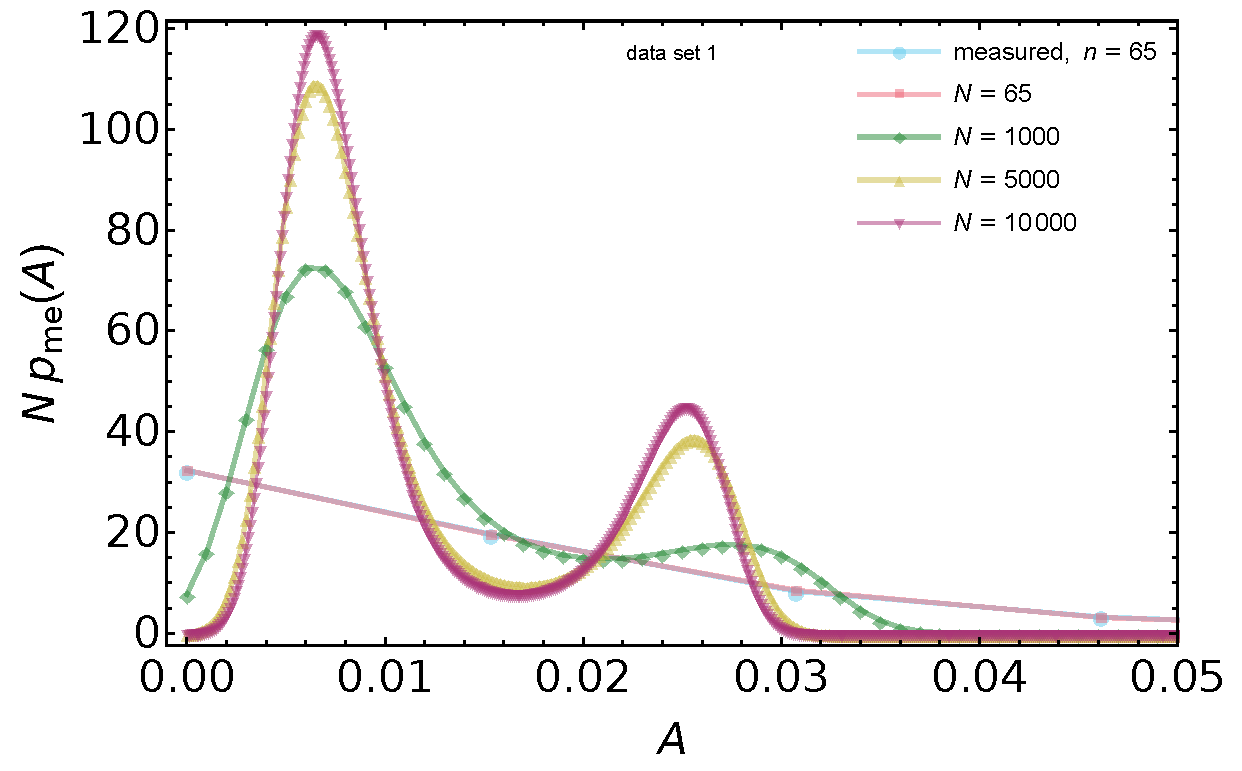
\includegraphics[width=\linewidth]{_scripts/paper_stensola_6mom_distributionsN_prior2.pdf}%
\\[3em]%
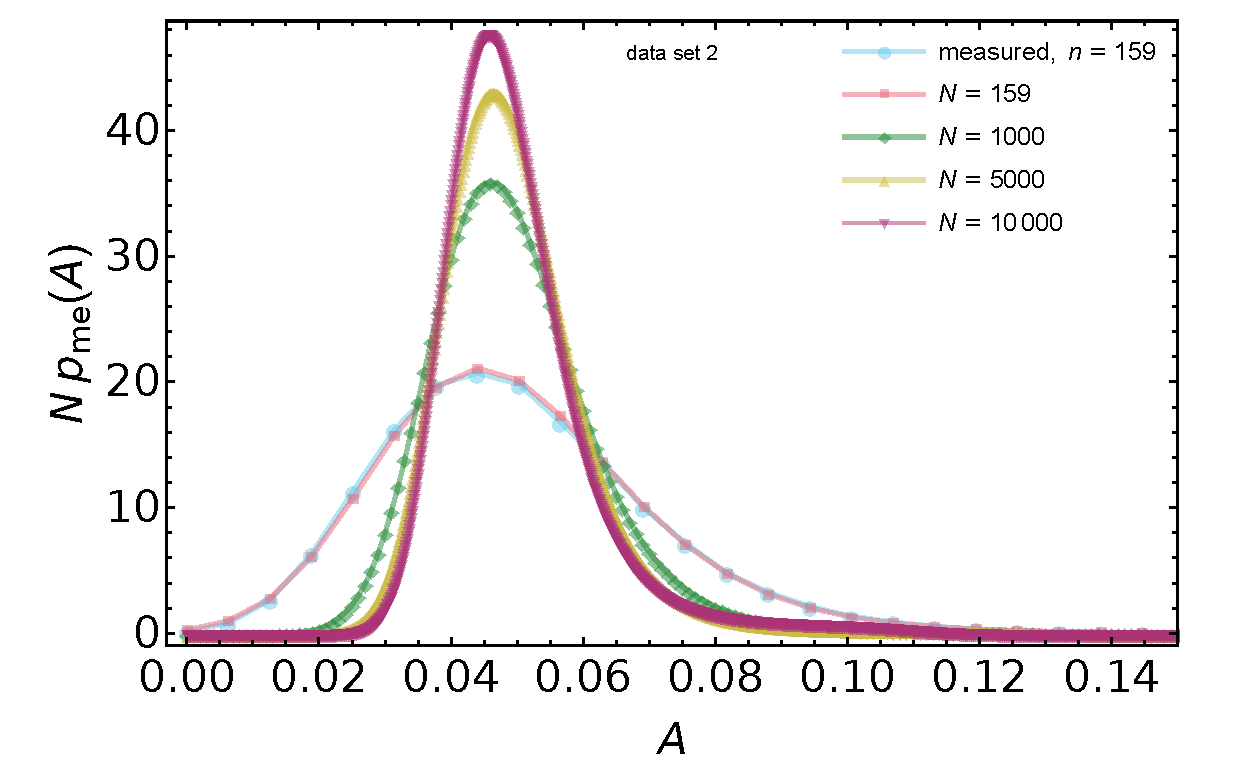
\includegraphics[width=\linewidth]{_scripts/paper_riehle_6mom_distributionsN_prior2.pdf}%
\caption{***}
\label{fig:plots_6mom}
\end{figure}
%maxent_solutions_different_moments_prior2_6moments.nb


The distribution for the full-network is sharper than the measured
frequency distribution for the sample; the sharper the larger $N$ is. Most
remarkably, it has two distinct low-activity modes for the first data set.
But also the second data set presents, upon closer inspection, a small
shoulder on the right of the mode, suggestive of two activity regimes. We
frame no hypotheses about the biological cause of these two modes (they
could stem from the presence of different kinds of cells or modules). These
features are clearly not present in the sample or in the maximum-entropy
distribution at the sample level. The application of the probability
calculus thus reveals interesting possible features of the full network.
\textcolor{white}{If you find this you can claim a postcard from us.}

\bigskip

To illustrate how our approach can be applied to studies of sufficient
statistics, \fig~\ref{fig:plots_2_4mom} shows the results for two
constrained moments (equivalent to constraining means and correlations
only) and for four constrained moments, with $N=10\,000$. In either data
set we obtain two very distinct distributions. For the first data set in
particular, four moments lead to a bimodal distribution, whereas two to a
unimodal one, showing that two moments would not be sufficient
statistics. For comparison, the two distributions obtained applying
maximum-entropy \emph{at the sample level} are shown as an inset in the
plot for the first data set: their differences aren't so glaring as in the
full-network application.
\begin{figure}[!p]
\centering
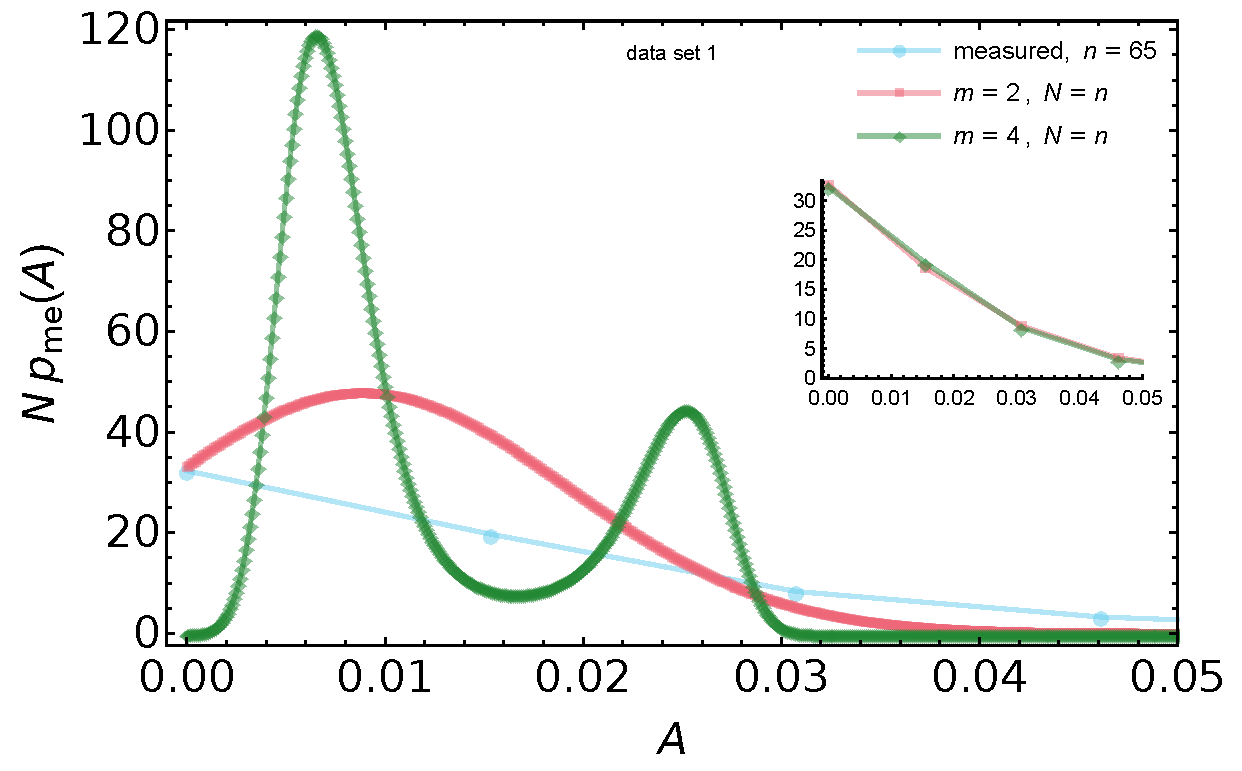
\includegraphics[width=\linewidth]{_scripts/paper2_stensola_twomom_distributions10000_prior2.pdf}%
\\[3em]%
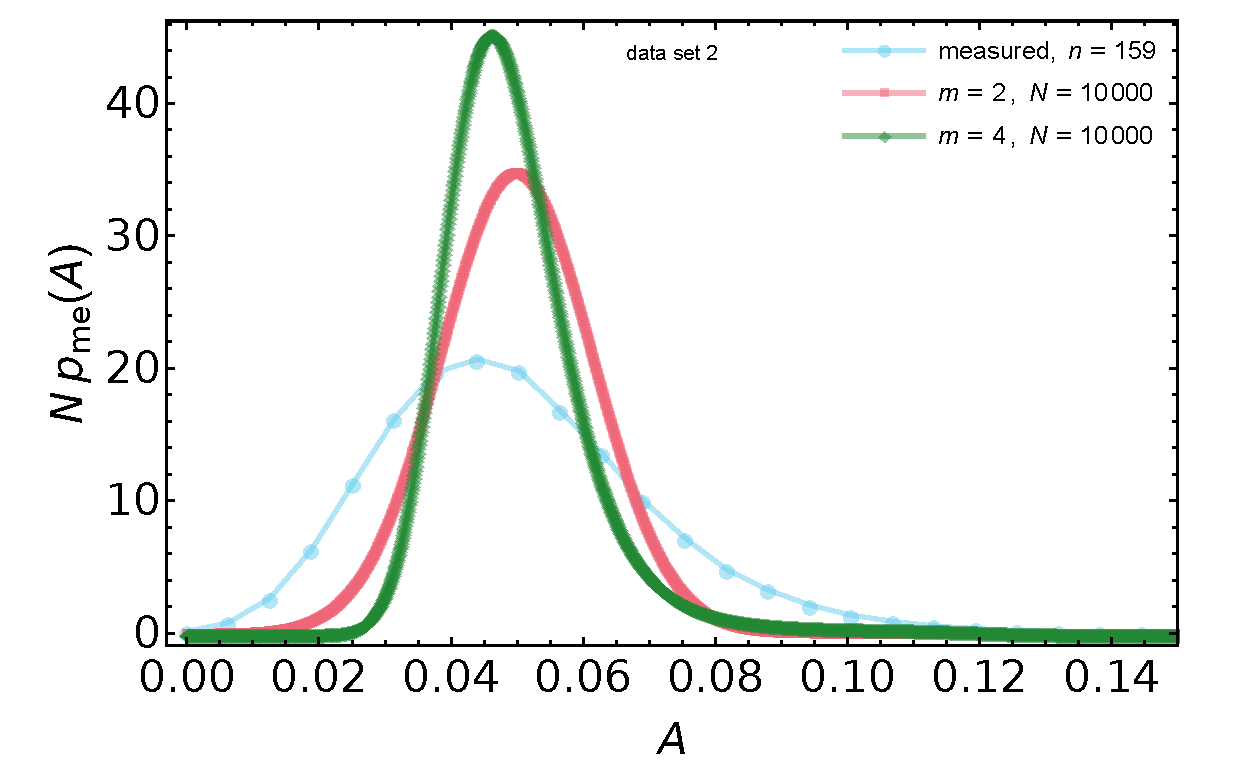
\includegraphics[width=\linewidth]{_scripts/paper_riehle_twomom_distributions10000_prior2.pdf}%
\caption{***}
\label{fig:plots_2_4mom}
\end{figure}
%maxent_solutions_different_moments_prior2_6moments.nb


\section{Marginalization to the sample level:\\ the issue with pairwise
  correlations and other statistics}
\label{sec:marginalization}

In the neurosciences the maximum-entropy method is often applied to
questions of sufficient statistics. In this section we discuss how our
proposed application bears on this kind of questions. For concreteness we
use an example with specific statistics: first and second moments
(equivalent to mean and correlations), versus first-to-fourth moments. But
our discussion holds for any  sets of statistics.

The question is as follows. We want to assess our degree of belief about
the frequencies of the activities of the sample, or about the sample
activity in a new time bin. For this assessment we should use all measured
data we have. But it sometimes happens that dropping part of the data --
for example, the measured third- and higher-order moments -- leaves our
assessment almost unchanged: the dropped data are \emph{informationally
  irrelevant}, or almost so. The remaining data -- for example, first and
second moments -- are \emph{informationally sufficient}. This informational
quasi-sufficiency is interesting because it may hint at peculiar biological
or physical mechanisms or dependencies.

We can approximately check how much some data are irrelevant by simply
dropping them from the conditional of our degree of belief, and see if the
latter changes appreciably. When our degree of belief is built with the
maximum-entropy method, we simply drop some of the data used as constraints
and see how the resulting distribution changes. For example, we may only
retain the first two moments (means and correlations) or the first four
moments. In the neurosciences this check is often done with maximum-entropy
distributions constructed \emph{for the sample}, ignoring the full network
it's sampled from.


% For example: does knowledge about
% third-order correlations change our state of uncertainty about network
% activity in an appreciable way, compared to knowledge about second-order
% correlations only? The method is used as follows to answer this question.
% We imagine to be ignorant of the measured frequency distribution for the
% network activity, and to know only up to second-order measured statistics,
% or up to third-order. Two maximum-entropy distributions are then built,
% constrained under the two sets of moments under comparison. Finally, the
% resulting distributions are compared with each other and with the measured
% frequency distribution. This recipe generalizes to any subsets of measured
% statistics, of course.

The method introduced in the present work reveals an issue with this
application at the sample level, however. The issue doesn't come from the method
itself but from a general fact of probability theory. If a probability
distribution has some sufficient statistics
\citep[\sect~4.5]{bernardoetal1994}{fortinietal2000}, then its marginals
\emph{cannot} have the same sufficient statistics, and vice versa, except
for trivial cases such as uniform distributions. This generally also holds
among different marginals: if a marginal has some sufficient statistics,
another won't have it. This impossibility is known in statistical
mechanics: marginals of Gibbs states aren't Gibbs states
\citep{maesetal1999}. Mathematically it corresponds to the general
impossibility of solving a system of $n$ equations in $m$ unknowns when
$n>m$ \citep[\sect~3.1]{portamanaetal2015}[\sect~3]{portamanaetal2018b}.

In our example this means that if means and pairwise correlations or the
first four moments are informationally sufficient for a particular sample
from a brain area, then they \emph{cannot} be sufficient for the full
network of neurons in that area, or for a different sample. Vice versa, if
we assume that they are informationally sufficient for the full network,
then we must expect them \emph{not} to be sufficient for any recorded
sample thereof. Now, questions about sufficient statistics are meant to be
addressed to a whole brain area, not just to some specific, casually
recorded sample. Thus, paradoxically, maximum-entropy methods applied at
the sample level give an answer opposite to the one we might think they're
giving.

Questions about informational sufficiency are therefore correctly addressed
by applying the maximum-entropy method at the full-network level. If a
comparison with the measured frequencies of the sample activities is
desired, then the marginal distribution to the sample size should be used.

\begin{figure}[!p]
\centering
\includegraphics[width=\linewidth]{_scripts/comparison_full.pdf}%
\\[3em]%
\includegraphics[width=\linewidth]{_scripts/comparison_marginals.pdf}%
\caption{***}
\label{fig:comparisons_marginals}
\end{figure}
%comparison_ME_sample_full_levels.nb
But does the application at the full-network level lead to appreciably
different results from that at the sample level? after all we're interested
in an approximate informational sufficiency, not in an analytically exact
one. A correct answer can only be given case by case;
\fig~\ref{fig:comparisons_marginals} gives a graphical answer to this
question in the case of our first data set. The upper plot shows the
maximum-entropy distributions for a full network of $10\,000$ neurons,
constructed from two moments (\textcolor{mygreen}{\textbf{--~--~--}}) and
from four moments (\textcolor{mypurpleblue}{\textbf{------}}). The lower plot
shows the maximum-entropy distributions for the sample, from two moments
(\textcolor{mygreen}{$\bm{\triangledown}$}) and from four moments
(\textcolor{mypurpleblue}{$\bm{\square}$}), and the distributions obtained by
marginalizing the full-network distribution to the sample size, from two
moments (\textcolor{mygreen}{$\bm{\blacktriangledown}$}) and from four
moments (\textcolor{mypurpleblue}{$\bm{\blacksquare}$}). The measured frequency
distribution (\textcolor{myred}{\LARGE$\bm{\bullet}$}) is also shown. We
note the following:
\begin{itemize}
\item The application to the full-network (upper plot) leads to two
  completely different distributions (even different number of modes);
  clearly the two sets of statistics are not even approximately equivalent
  for inferential purposes.
\item The application at the sample level leads to deceivingly similar
  distributions (\textcolor{mygreen}{$\bm{\triangledown}$} and
  \textcolor{mypurpleblue}{$\bm{\square}$}), which can only be distinguished on a
  logarithmic scale. This could lead to the erroneous conclusion that the
  two statistics are approximately equivalent.
\item The difference between marginals from the full-network distribution
  and the distributions obtained at the sample level (filled vs empty
  markers) is larger than the difference between different statistics
  (triangles vs squares).
\item The marginals of the application to the full network are closer to
  the measured frequencies than the distributions obtained at the sample
  level (although this closeness is not a valid criterion for their
  goodness).
\end{itemize}
Therefore, the maximum-entropy application at the sample level and at the
full-network level lead to different results; the latter is not only more
meaningful but also superior because it shows clearly the different
informational sufficiency of the two sets of statistics.


\section{The full-network size $N$}
\label{sec:N}

The calculations and conclusions presented in the preceding sections depend
on the size of the full network, $N$. The full network can't be the whole
brain, of course; that would be silly. How large can $N$ be?

The crucial point is formula~\eqref{eq:equal_m_factorialmoments}, on which
our method is based, and which asserts the equality of the factorial
moments of the full network and its sample, (or, equivalently, asserting
that the power moments for the one are linear functions of the power
moments for the other). This formula is only valid if our beliefs about the
activity of the sample  $\pxx(\ya)$ and that of the full network
$\pxx(\yA)$ are related by a hypergeometric distribution:
\begin{equation}
  \label{eq:hypergeometric_relation}
    \pxx(\ya)=
  \binom{n}{n\ya}\;\binom{\yNv-n}{\yNv \yA-n\ya}\;\binom{\yNv}{\yNv \yA}^{-1}
\;\pxx(\yA).
\end{equation}
This is a relation of \enquote{drawing without replacement}
\citep[\chap~3]{jaynes1994_r2003}[\sect~4.8.3]{ross1976_r2010}[\sect~II.6]{feller1950_r1968}.
In other words, $N$ must be such that we equally believe other samples of
size $n$ could have been recorded by the electrodes or the probe used. This
is indeed what we stated in \sect~\ref{sec:model}.

This requirement delimits an area around the probe. Its number of neurons
depends on the animal species and on the brain region from which the
recording was made, as the neuron density can be very different. It's
practically impossible to specify the exact number of neurons, but its
order of magnitude is enough for making qualitative inferences. As we'll
discuss in the next section, even if the exact number were known the
maximum-entropy distribution ought still to be interpreted qualitatively.

It would be possible to derive a distribution $\pxx(A)$ for the full
network based on an unknown $N$, by  expressing our belief distribution
$\pxx(N)$ about $N$ and using this to marginalize $N$ out:
\begin{equation}
  \label{eq:marginalize_N}
  \pxx(A \| \text{$N$ \small unknown}) = \sum_{N} \px(\yA \| N)\;\pxx(N).
\end{equation}
But this would be overkill, owing to the qualitative character of the
maximum-entropy distribution constructed with exact $N$.












\section{Summary and discussion}
\label{sec:summary_discussion}

These results caution us against taking maximum-entropy solutions too
literally. The full probabilistic analysis allows us to see more clearly
the extent of our uncertainty and to make better-informed guesses.

\clearpage
\hrule
OLD TEXT
\hrule

\section{Mathematical development}
\label{sec:maths_development}

\begin{subequations}
  \label{eq:all_equal_expectations_poll}
\begin{equation}
  \label{eq:equal_factorialmoments_polls}
  \begin{split}
  \E\condt[\big]{\tfrac{s\;(s-1)}{n\;(n-1)}}{\yH} &= 
  \E\condt[\big]{\tfrac{S\;(S-1)}{N\;(N-1)}}{\yH},\\
  \E\condt[\big]{\tfrac{s\;(s-1)\;(s-2)}{n\;(n-1)\;(n-2)}}{\yH} &= 
  \E\condt[\big]{\tfrac{S\;(S-1)\;(S-2)}{N\;(N-1)\;(N-2)}}{\yH},
  \\
  \text{and in general}\quad
  \E\condt[\big]{\tbinom{s}{r}\;\tbinom{n}{r}^{-1}}{\yH} &=
  \E\condt[\big]{\tbinom{S}{r}\;\tbinom{N}{r}^{-1}}{\yH},
  \quad r<N.
\end{split}
\end{equation}

Note that from the first $r$ factorial moments we can calculate the first
$r$ power moments and vice versa; but the simple equalities above don't
hold for the power moments \citep[\sect~A]{portamanaetal2015}.

\begin{equation}
  \label{eq:relation_ps_pS}
  \pf(s \| \yH) = \sum_{S} \binom{n}{s}\;\binom{N-n}{S-s}\;\binom{N}{S}^{-1}\;
  \pf(S \| \yH).
\end{equation}
\end{subequations}


Suppose we have recorded the firing activity of a hundred neurons,
sampled from a particular brain area. What are we to do with such data?
Gerstein \etal\ \citey{gersteinetal1985} posed this question very
tersely (our emphasis):
\begin{quote}\small
  The principal conceptual problems are (1) \emph{defining cooperativity or
    functional grouping} among neurons and (2) \emph{formulating
    quantitative criteria} for recognizing and characterizing such
  cooperativity.
\end{quote}
These questions have a long history, of course; see for instance the 1966
review by Moore \etal\
\citey{mooreetal1966}. % This scenario is a concrete possibility
% thanks to recent electrophysiological techniques \citep{berenyietal2014}.
The neuroscientific literature has offered several mathematical definitions
of \enquote{cooperativity} or \enquote{functional grouping} and criteria to
quantify it.

One such quantitative criterion relies on the \me\ or relative-\me\ method
\citep{jaynes1957,jaynes1963,hobsonetal1973,sivia1996_r2006,meadetal1984}.
This criterion has been used in neuroscience at least since the 1990s,
applied to data recorded from brain areas as diverse as retina and motor
cortex
\citep{mackay1991,martignonetal1995,bohteetal2000,amarietal2003,schneidmanetal2006,shlensetal2006,mackeetal2009b,roudietal2009c,tkaciketal2009,gerwinnetal2009,mackeetal2011,mackeetal2011b,ganmoretal2011,granotatedgietal2013,tkaciketal2014b,moraetal2015,shimazakietal2015},
and it has been subjected to mathematical and conceptual scrutiny
\citep{tkaciketal2006,roudietal2009,roudietal2009b,barreiroetal2010,barreiroetal2010b,mackeetal2013,rostamietal2016_r2017}.

\enquote{Cooperativity} can be quantified and characterized with \me\
methods in several ways. The simplest way roughly proceeds along the
following steps. Consider the recorded activity of a sample of $n$ neurons.
\begin{enumerate}
\item The activity of each neuron, a continuous signal, is divided into $T$
  time bins and binarized in intensity, and thus transformed into a
  sequence of digits \enquote{$0$}s (inactive) and \enquote{$1$}s (active)
  \citep[\cf][]{caianiello1961,caianiello1986}.

  Let the variable $\yav_i(t)\in\set{0,1}$ denote the activity of the $i$th
  sampled neuron at time bin $t$. Collectively denote the $n$ activities
  with $\yaa(t) \defd \bigl(\yav_1(t),\dotsc,\yav_n(t)\bigr)$. The
  network-averaged activity at that bin is
  $\ya(t) \defd \sum_i \yav_i(t)/n$. If we count the number of distinct
  pairs of active neurons at that bin we combinatorially find
  $\tbinom{n\ya(t)}{2}\equiv n\ya(t)\,[n\ya(t)-1]/2$. There can be at
  most $\tbinom{n}{2}$ simultaneously active pairs, so the
  network-averaged pair activity is
  $\av{\yaa \yaa}(t) \defd \tbinom{n}{2}^{-1}\tbinom{n\ya(t)}{2}$. With some
  combinatorics we see that the network-averaged activity of $m$-tuples
  of neurons is
  \begin{equation}
    \label{eq:products_intermsof_average}
    \av{\underbrace{\yaa\dotsm\yaa}_{\text{$m$ terms}}}(t)
    = \binom{n}{m}^{-1}\binom{n\ya(t)}{m}.
  \end{equation}
  
  For brevity let us agree to simply call \enquote{activity} the average
  $\ya$, \enquote{pair-activity} the average $\av{\yaa \yaa}$, and so on.

\item Construct a sequence of relative-\me\ distributions for the activity
  $\ya$, using this sequence of constraints:
  \begin{itemize}
  \item the time average of the activity: $\tav{\ya} \defd \sum_t\ya(t)/T$;
  \item the time averages of the activity and of the pair-activity
    $\tav{\av{\yaa \yaa}} \defd \sum_t\av{\yaa \yaa}(t)/T$;
  \item \ldots
  \item the time averages of the activity, of the pair-activity, and so on, up
    to the $k$-activity.
  \end{itemize}
  Call the resulting distributions $p_1(\ya), p_2(\ya),\dotsc,p_k(\ya)$.
  The time-bin dependence is now absent because these distributions can be
  interpreted as referring to any one of the time bins $t$, or to a new
  time bin (in the future or in the past) containing new data.

  We also have the empirical frequency distribution of the total activity,
  $f(\ya)$, counted from the time bins.

\item Now compare the distributions above with one another and with the
  frequency distribution, using some probability-space distance like the
  relative entropy or discrimination information
  \citep{kullback1987,jaynes1963,hobson1969,hobsonetal1973}. If we find,
  say, that such distance is very high between $p_1$ and $f$, very low
  between $p_2$ and $f$, and is more or less the same between all $p_m$ and
  $f$ for $m \ge 2$, then we can say that there is a \enquote{pairwise
    cooperativity}, and that any higher-order cooperativity is just a
  reflection or consequence of the pairwise one. The reason is that the
  information from higher-order simultaneous activities did not lead to
  appreciable changes in the distribution obtained from pair activities.
\end{enumerate}
The protocol above needs to be made precise by specifying various
parameters, such as the width of the time bins or the probability
distance used.

We hurry to say that the description just given is just \emph{one} way to
quantify and characterize cooperativity and functional grouping, not
\emph{the only} way. It can surely be criticized from many points of view.
Yet, it is quantitative and bears a more precise meaning than an undefined,
vague notion of \enquote{cooperativity}. Two persons who apply this
procedure to the same data will obtain the same numbers. Different
protocols can be based on the \me\ method, for instance protocols that take
into account the activities or pair activities of specific neurons rather
than network averages, or even protocols that take into account time
dependence.

The purpose of the present work is not to assess the merits of \me\ methods
with respect to other methods. Its main purpose is to show that there is a
problem in the way the \me\ method itself, as sketched above, is applied to
the activity of the recorded neurons. We believe that this problem is at
the root of some quirks about this method that were pointed out in the
literature \citep{roudietal2009b}. This problems extends also to more
complex versions of the method, possibly except versions that use
\enquote{hidden} neurons
\citep{smolensky1986,kulkarnietal2007,huang2015,dunnetal2017}. The problem is
that the recorded neurons are a \emph{sample} from a larger, unrecorded
network, but the \me\ method as applied above is treating them as
isolated from the rest of the brain. Hence, the results it provides cannot
be rightfully extrapolated. We will give a mathematical proof of this. Let
us first analyse this issue in more detail.

Suppose that the neurons were recorded with electrodes covering an area of
some square millimetres \citep[\cf][]{berenyietal2014}. This recording is a
sample of the activity of the neuronal network under the recording
device, which can amount to tens of thousands of neurons
\citep{abeles1991}. We could even consider the recorded neurons as a sample
of a brain area more extended than the recording device.

The characterization of the cooperativity of the recorded sample would have
little meaning if we did not expect its results to generalize to a larger,
unrecorded network -- at the very least the network under the
recording device. In other words, we expect that the conclusions drawn with
the \me\ methods about the sampled neurons should somehow extrapolate to
unrecorded neurons in some larger area, from which the recorded neurons
were sampled. In statistical terms we are assuming that the recorded
neurons are a \emph{representative sample} of some larger neuronal
network. Probability theory tells us how to make inferences from a
sample to the larger network from which it is sampled \parentext{see
  references below}.

We can apply the \me\ method to the sample, as described in the above
protocol, to generate probability distributions for the activity of the
sample. But, given that our sample is representative of a larger
network, we can also apply the \me\ method to the larger (unrecorded)
network. The constraints are the same: the time averages of the sampled
data, since they constitute representative data about the larger network
as well. The method thus yields a probability distribution for the larger
network, and the distribution for the sample is obtained by
marginalization. The problem is that \emph{the distributions obtained from
  these two applications differ}. Which choice is most meaningful?

In this work we develop the second way of applying the \me\ method, at the
level of the larger network, and show that its results differ from the
application at the sample level. We also consider the case where the size
of the larger network is unknown.

To apply the \me\ method to the larger, unsampled network, it is
necessary to use probability relations relevant to sampling
\citep{ghoshetal1997}[parts~I,
VI]{freedmanetal1978_r2007}[\chap~8]{gelmanetal1995_r2014}[\chap~3]{jaynes1994_r2003}.
The relations we present are well-known in survey sampling and in the
pedagogic problem of drawing from an urn without replacement, yet they are
somewhat hard to find explicitly written in the neuroscientific literature.
We present and discuss them in the next section. A minor purpose of this
paper is to make these relations more widely known, because they can be
useful independently of \me\ methods.


The notation and terminology in the present work follow ISO and ANSI standards
\citep{iso1993,ieee1993,nist1995,iso2006,iso2006b} but for the use of the
comma \enquote{,} to denote logical conjunction. Probability notation
follows Jaynes \citep{jaynes1994_r2003}. By \enquote{probability} we mean a
degree of belief which \enquote{would be agreed by all rational men if
  there were any rational men} \citep{good1966}.



\section{Probability relations between network and  sample}
\label{sec:prob_samples}

We have already introduced the notation for the sample neurons. We
introduce an analogous notation for the $\yNv$ neurons constituting the
larger network, but using the corresponding capital letters:
$\yAv_{i}(t)$ is the activity of the $i$th neuron at time bin $t$,
$\yA(t) \defd \sum_{i} \yAv_{i}(t)/\yNv$ is the activity at that
bin averaged over the larger network, and so on.

The probability relations between sample and larger network are valid at
every time bin. As we mentioned above, the \me\ distribution refers to any
time bin or to a new bin. For these reasons we will now omit the time-bin
argument \enquote{$(t)$} from our expressions. 

% Probabilities refer to statements about the quantities we observe. We use
% the standard notation:
% \begin{equation}
%   \label{eq:notation_statements}
%   \begin{aligned}
%     &\text{\enquote{$\yXv_{\iota} = \yAv_{\iota}$} 
%       stands for \enquote{the activity of the $\iota$th neuron is $\yAv_{\iota}$}},
%     \\
%     &\text{\enquote{$\yXf = \yA$} 
%       stands for \enquote{the (network-averaged) activity of the neurons is $\yA$}},
%     \\
%     &\text{\enquote{$\yxv_i = \yav_i$} 
%       stands for \enquote{the activity of the $i$th sample neuron is $\yav_i$}},
%   \end{aligned}
% \end{equation}
% and similarly for other quantities.


If $\yHc$ denotes our state of knowledge -- the evidence and assumptions
backing our probability assignments -- our uncertainty about the full
activity of the larger network is expressed by the joint probability
distribution
\begin{equation}
  \label{eq:joint_plaus}
  \pf(\yAv_1, \yAv_2, \dotsc, \yAv_\yNv \| \yHc)
  \quad\text{or}\quad
\pf(\yAA \| \yHc), \quad \yAA \in \set{0,1}^\yNv.
\end{equation}
Our uncertainty about the state of the sample is likewise expressed by
\begin{equation}
  \label{eq:sample_plaus}
  \pf(\yav_1, \yav_2, \dotsc, \yav_n \| \yHc) \quad\text{or}\quad
\pf(\yaa \| \yHc), \quad \yaa \in \set{0,1}^n.
\end{equation}

\bigskip

The theory of statistical sampling is covered in many excellent texts, for
example Ghosh \amp\ Meeden \citey{ghoshetal1997} or Freedman, Pisani, \amp\
Purves \citey[parts~I, VI]{freedmanetal1978_r2007}; summaries can be found
in Gelman \etal\ \citey[\chap~8]{gelmanetal1995_r2014} and Jaynes
\citey[\chap~3]{jaynes1994_r2003}.

We need to make an initial probability assignment for the state of the full
network before any experimental observations are made. This initial
assignment will be modified by our experimental observations, and these can
involve just a sample of the network. Our state of knowledge and initial
probability assignment should reflect that samples are somehow
representative of the whole network.

In this state of knowledge, denoted $\yH$, we know that the neurons in the
network are biologically or functionally similar, for example in
morphology or the kind of input or output they receive or give. But we are
completely ignorant about the physical details of the individual neurons.
Our ignorance is therefore symmetric under permutations of neuron
identities. This ignorance is represented by a probability distribution
that is symmetric under permutations of neuron identities; such a
distribution is usually called \emph{finitely exchangeable}
\citep{ericson1969}[\chap~1]{ghoshetal1997}. We stress that this
probability assignment is just an expression of the symmetry of our
\emph{ignorance} about the state of the network, not an expression of
some biologic or physical symmetry or identity of the neurons.

The \emph{representation theorem for finite exchangeability} states that,
in the state of knowledge $\yH$, the symmetric distribution for the full
activity is completely determined by the distribution for its
network-average:
\begin{equation}
  \label{eq:joint_plaus_N_homog}
  \pf(\yAA \|  \yH) \equiv
  \sum_{\yA}\pf(\yAA \| \yA, \yH)\,
  \pf(\yA \| \yH) =
  \binom{\yNv}{\yNv\yA}^{-1} \pf(\yA \| \yH).
\end{equation}
The equivalence on the left is just an application of the law of total
probability; the equality on the right is the statement of the theorem.
This result is intuitive: owing to symmetry, we must assign equal
probabilities to all $\tbinom{\yNv}{\yNv\yA}$ activity vectors with
$\yNv\yA$ active neurons; the probability of each activity vector is
therefore given by that of the average activity divided by the number of
possible vector values. Proof of this theorem and generalizations to
non-binary and continuum cases are given by de~Finetti
\citey{definetti1959b}, Kendall \citey{kendall1967}, Ericson
\citey{ericson1976}, Diaconis \amp\ Freedman
\citey{diaconis1977,diaconisetal1980}, Heath \amp\ Sudderth
\citey{heathetal1976}.

Our uncertainties about the full network and the sample are connected
via the conditional probability
\begin{equation}
  \label{eq:conditional_hypergeometric}
  \pf(\ya \|\yA, \yH)=
  \binom{n}{n\ya}\binom{\yNv-n}{\yNv \yA-n\ya}\binom{\yNv}{\yNv \yA}^{-1}
  \defs \ypp_{\ya\yA},
\end{equation}
which is a hypergeometric distribution, typical of \enquote{drawing without
  replacement} problems. The combinatorial proof of this expression is in
fact the same as for this class of problems
\citep[\chap~3]{jaynes1994_r2003}[\sect~4.8.3]{ross1976_r2010}[\sect~II.6]{feller1950_r1968}.

Using the conditional probability above we obtain the probability for the
activity of the sample:
\begin{gather}
  \label{eq:subpop_average}
  \pf(\ya \| \yH) = \sum_{\yA}
  \pf(\ya \|\yA, \yH)\,
  \pf(\yA \| \yH)
  = 
  \sum_{\yA}
  \ypp_{\ya\yA}\,
  \pf(\yA \| \yH).
\end{gather}
It should be proved that the probability distribution for the full activity
of the sample is also symmetric and completely determined by the
distribution of its network-averaged activity:
\begin{equation}
  \label{eq:marginal}
  \pf(\yaa \| \yH) = \binom{n}{n\ya}^{-1} \pf(\ya \| \yH).
\end{equation}
This is intuitively clear: our initial symmetric ignorance should also
apply to the sample. The distribution for the
sample~\eqref{eq:subpop_average} indeed satisfies the same representation
theorem~\eqref{eq:joint_plaus_N_homog} as the distribution for the full
network.

The conditional probability
$\pf(\ya \|\yA, \yH) \equiv \ypp_{\ya \yA}$, besides
relating the distributions for the network and sample activities via
marginalization, also allows us to express the expectation value of any
function of the sample activity, $\yg_{\ya}$, in terms of the distribution
for the full network, as follows:
\begin{equation}
  \label{eq:pullback_P}
  \E(\yg\|I)
  \equiv
  \sum_{\ya} \yg_{\ya}\,\pf(\ya \| \yH)
  =
  \sum_{\ya} \yg_{\ya} \sum_{\yA} \ypp_{\ya\yA}\,\pf(\yA \| \yH)
  =%{}\\
  \sum_{\yA} \bigl( \tsum_{\ya} \yg_{\ya}  \ypp_{\ya\yA} \bigr)\,
  \pf(\yA \| \yH),
%  =
%  \sum_{N\yA=0}^N \sum_{n\ya=0}^n f(\ya)\ypp_{\ya\yA}\,\p(\yXf=\yA \| \yH)
%  \equiv  \expeb{\yg^*}.
\end{equation}
where the second step uses \eqn~\eqref{eq:subpop_average}. The last
expression shows that the expectation of the function $\yg_{\ya}$ is equal to
the expectation of the function
$\yg^*(\yA) \defd \sum_{\ya} \yg_{\ya}\,\ypp_{\ya\yA}$.

\bigskip

The final expression in \eqn~\eqref{eq:pullback_P} is important for our
\me\ application: the requirement that the function $\yg$, defined for the
sample, have a  value $\yc$ obtained from observed data,
\emph{translates into a linear constraint for the distribution of the full
  network}:
\begin{equation}
  \label{eq:constraint_extended}
  \yc = \E(\yg \| \yH) \equiv \sum_{\yA} \bigl( \tsum_{\ya} \yg_{\ya}  \ypp_{\ya\yA} \bigr)\;
  \pf(\yA \| \yH).
\end{equation}

In particular, when the function $\yg$ is the $m$-activity of the sample,
$\yg_{\ya} = \sav{\yaa\dotso\yaa} \equiv \binom{n\ya}{m}/\binom{n}{m}$, we
find
\begin{multline}
  \label{eq:expe_products}
%  \label{eq:pullback_m_expectations}
%  \ypp^*\colon \sav{\underbrace{\yx \dotsm \yx}_{\text{$m$ factors}}}
%  \mapsto
    % \bigl( \sav{\underbrace{\yx \dotsm \yx}_{\text{$m$ factors}}}\bigr)^* =
    % \av{\underbrace{\yX \dotsm \yX}_{\text{$m$ factors}}},
    % \\[2\jot]
    % \expe{\sav{\underbrace{\yx \dotsm \yx}_{\text{$m$ factors}}} \| \yH} =
    % \expe{\av{\underbrace{\yX \dotsm \yX}_{\text{$m$ factors}}} \| \yH}
  \E(\sav{\underbrace{\yaa \dotsm \yaa}_{\text{$m$ factors}}} \| \yH)
\equiv
    % \\[2\jot]
    % {}
    % \frac{(n-m)!}{n!}
    \sum_{\ya} %m!\,
    \binom{n}{m}^{-1}
    \binom{n \ya}{m}\, \pf(\ya \| \yH)
    % \sum_{N \yA=0}^N %m!\,
    % \binom{N-m}{N \yA-m} \binom{N}{N \yA}^{-1} \p(\yXf=\yA \| \yH)
    ={}\\
    \binom{\yNv}{m}^{-1}
    % \frac{(N-m)!}{N!}
    \sum_{\yA} %m!\,
    \binom{\yNv \yA}{m}\, \pf(\yA \| \yH)
\equiv    \E(\av{\underbrace{\yAA \dotsm \yAA}_{\text{$m$ factors}}} \| \yH),
\end{multline}
that is, \emph{the expected values of the $m$-activities of the sample and
  of the full network are equal}. The proof of the middle equality uses
the expression for the $m$th factorial moment of the hypergeometric
distribution and can be found in \textcite{potts1953}. Similar relations
can be found for the raw moments $\E(\ya^m)$ and $\E(\yA^m)$, which
can be written in terms of the product expectations using
\eqn~\eqref{eq:products_intermsof_average}.

Thus, in a \me\ application, when we require the expectation of the
$m$-activity of a sample to have a particular value, we are also
requiring  the expectation of the $m$-activity of the full network to
have the same value.

\bigskip


\begin{figure}[!b]
\centering
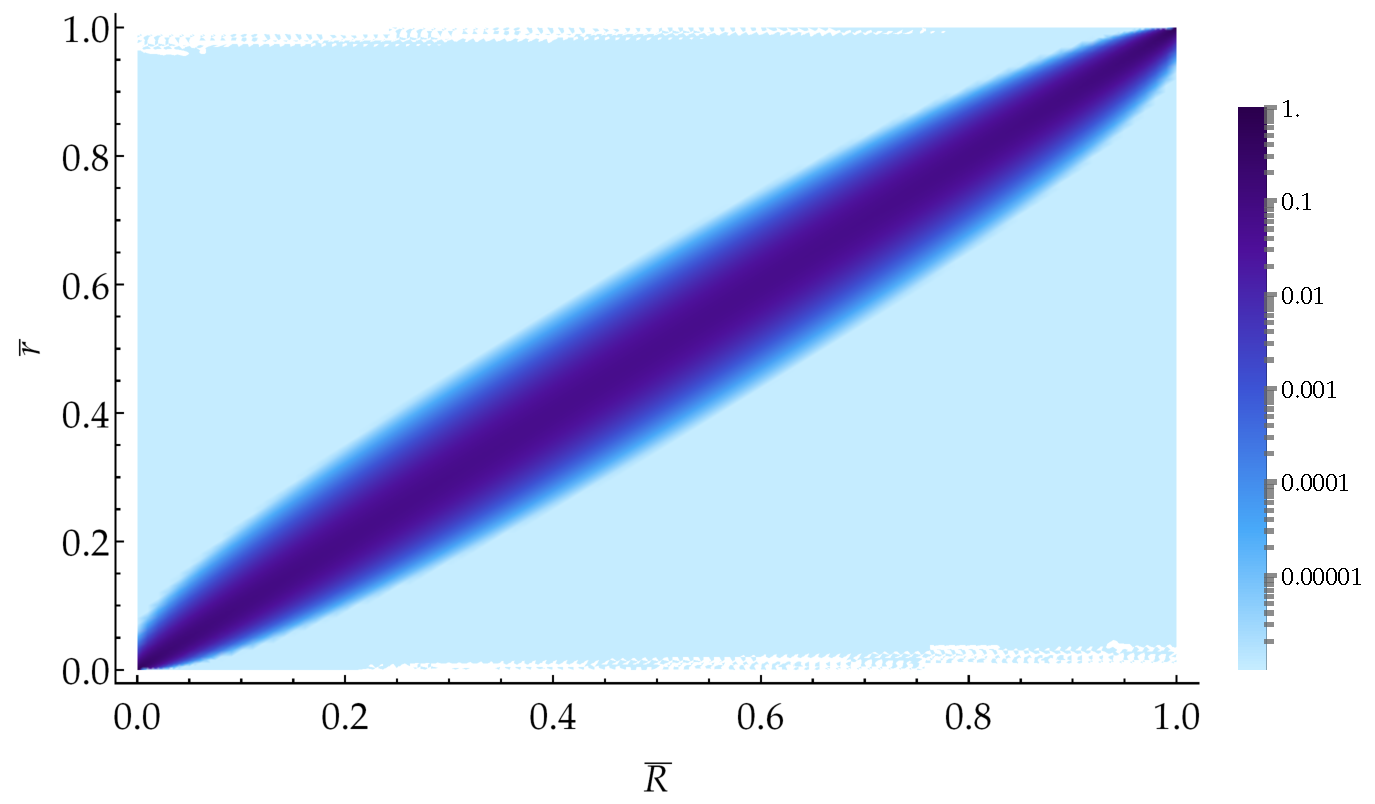
\includegraphics[width=\linewidth]{pop_sample_projection3.pdf}%
\caption{Log-density plot of the hypergeometric distribution
  $%\pf(\ya \|\yA, \yH)=
\ypp_{\ya\yA} \defd  \raisebox{0pt}[0pt][1ex]{}\binom{n}{n\ya}\binom{\yNv-n}{\yNv \yA-n\ya}\binom{\yNv}{\yNv \yA}^{-1}$ for $\yNv=5000$, $n=200$. (Band artifacts may appear in the
  colourbar depending on your \textsc{pdf} viewer.)}
\label{fig:hypergeom_proj}
\end{figure}%hypergeometric_identity.nb
These expectation equalities between sample and full network should not
be surprising: we intuitively \emph{expect} that the proportion of coloured
balls sampled from an urn should be roughly equal to the proportion of
coloured ball contained in the urn. The formulae in the present section
formalize and mathematically express our intuition. The hypergeometric
distribution $\ypp_{\ya\yA}$ plays an important role in this
formalization. A look at its plot, \fig~\ref{fig:hypergeom_proj}, reveals
that it is a sort of \enquote{fuzzy identity transformation}, or fuzzy
Kronecker delta, between the $\yA$-space $\set{0,\dotsc,\yNv}$ and
$\ya$-space $\set{0,\dotsc,n}$. From \eqn~\eqref{eq:marginal} we thus have
that
\begin{equation}
  \label{eq:roughly_equal_nN}
  \pf(\ya=a \|\yH) \approx \pf(\yA=a \|\yH),\qquad
\E[\yg_{\ya} \|\yH] \approx \E[\yg_{\yA} \|\yH],
\end{equation}
where $\yg$ is any smooth function defined on $\clcl{0,1}$. These approximate
equalities express the intuitive fact that \emph{our uncertainty about the
  sample is representative of our uncertainty about the network and
  about other samples}, and vice versa. When $n=\yNv$, $\ypp_{\ya\yA}$
becomes the identity matrix and the approximate equalities above become
exact -- of course, since we have sampled the full network.

But the approximate equalities above may miss important features of the two
probability distributions. In the next section we will in fact emphasize
their differences. If the distribution for the network average $\yA$ is
bimodal, for example, the bimodality can be lost in the distribution for
the sample average $\ya$, owing to the coarsening effect of
$\ypp_{\ya\yA}$.

% They should be contrasted with the limits
% $\pf(\yxs=a) \to \pf(\yXf=a)$ and $\expeb{\yg_{\yxs}} \to \expeb{\yg_{\yXf}}$, as
% $n\to \yNv$, do: these limits are trivially, universally valid because the
% sample becomes the full network as $n\to \yNv$. In particular, these limits
% hold even in cases where the conditional probability
% $\pf(\yxs = \ya \|\yXf=\yA)$ is not a fuzzy identity, our uncertainties
% about sample and about network can differ wildly, and the approximate
% equalities~\eqref{eq:roughly_equal_nN} do not hold.



\section{Maximum-entropy: sample level \vs\ full-network level}
\label{sec:specific_initial_probability}

In the previous section we have seen that observations about a sample can
be used as constraints on the distribution for the activity of the full
network. Let us use such constraints with the \me\ method. Suppose that
we want to constrain $m$ functions of the sample activity, vectorially
written $\yg \defd (c_1,\dotsc,c_m)$, to $m$ values
$\yc \defd (\widehat{c}_1,\dotsc,\widehat{c}_m)$. These functions are typically $k$-activities
$\sav{\yaa\dotso \yaa}$, and the values are typically the time averages of
the observed sample, as discussed in \sect~\ref{sec:intro}:
$\yc = \sum_t \yg[\ya(t)]/T$.

Let us apply the relative-\me\ method \citep{sivia1996_r2006,meadetal1984}
directly to sampled neurons; denote this approach by $\yHb$. Then we apply
the method to the full network of neurons, most of which are unsampled;
denote this approach by $\yHa$.

Applied directly to the sampled neurons, the method yields the distribution
\begin{equation}
  \label{eq:app_maxent_sample}
  \pf(\ya \|\yHb)
  =\frac{1}{\yk(\yl)}\,
  \binom{n}{n\ya}
  \exp[\yl\T \yg_{\ya}]
\end{equation}
where $\yk(\yl)$ is a normalization constant. The binomial in front of the
exponential appears because we must account for the multiplicity by which
the network-average activity $\ya$ can be realized: $\ya=0$ can be
realized in only one way (all neurons inactive), $\ya=1/n$ can be realized
in $n$ ways (one active neuron out of $n$), and so on. This term is analogous to
the \enquote{density of states} in front of the Boltzmann factor in
statistical mechanics \citep[\chap~16]{callen1960_r1985}. The $m$ Lagrange
multipliers $\yl\defd (l_1,\dotsc,l_m)$ must satisfy the $m$ constraint
equations
\begin{equation}
  \label{eq:app_maxent_sample_constraints}
  \yc = \E(\yg \|\yHb) \equiv
  \frac{1}{\yk(\yl)}\sum_{\ya}  \yg_{\ya} \binom{n}{n\ya}
  \exp[\yl\T \yg_{\ya}].%, \qquad k=1,\dotsc,m.
\end{equation}

Applied to the full network, using the constraint
expression~\eqref{eq:constraint_extended} derived in the previous section,
the method yields the distribution for the full-network activity
\begin{equation}
  \label{eq:app_maxent_pop}
  \pf(\yA \| \yHa)  = \frac{1}{\yK(\yll)}\,
  \binom{\yNv}{\yNv \yA}\,\exp\bigl(\yll\T
  \tsum_{\ya} \yg_{\ya}\ypp_{\ya\yA}\bigr).
\end{equation}
The $m$ Lagrange multipliers $\yll\defd (\lambda_1,\dotsc,\lambda_m)$ must
satisfy the $m$ constraint equations
\begin{equation}
  \label{eq:app_maxent_pop_constraints}
  \yc = \E(\yg \|\yHa)\equiv %{}\\
 \frac{1}{\yK(\yll)}\sum_{\ya} \sum_{\yA} \yg_{\ya} \ypp_{\ya \yA}
\,
  \binom{\yNv}{\yNv \yA}\,\exp\bigl(\yll\T
  \tsum_{\ya} \yg_{\ya}\ypp_{\ya\yA}\bigr).
%  \\ k=1,\dotsc,m.
\end{equation}

We obtain the distribution for the sample activity by marginalization, using
\eqn~\eqref{eq:marginal}:
\begin{equation}
  \label{eq:app_maxent_pop_marg}
  \pf(\ya \| \yHa)  = \frac{1}{\yK(\yll)}\, 
  \sum_{\yA} \ypp_{\ya \yA}
\,
  \binom{\yNv}{\yNv \yA}\,\exp\bigl(\yll\T
  \tsum_{\ya} \yg_{\ya}\ypp_{\ya\yA}\bigr).
\end{equation}

The distributions for the sample activity,
\eqns~\eqref{eq:app_maxent_pop_marg} and \eqref{eq:app_maxent_sample},
obtained with the two approaches $\yHb$ and $\yHa$, are different. From the
discussion in the previous section we expect them to be vaguely similar;
yet they cannot be exactly equal, because their equality would require the
$2m$ quantities $\yll$ and $\yl$ to satisfy the constraint equations
\eqref{eq:app_maxent_pop_constraints} and
\eqref{eq:app_maxent_sample_constraints}, and in addition also the $n$
equations $\pf(\ya \| \yHa) = \pf(\ya \| \yHb)$,
$\ya=1/n,\dotsc,1$ (one equation is taken care of by the normalization of
the distributions). We would have a set of $2m+n$ equations in $2m$
unknowns.

Hence, \emph{the applications of \me\ at the sample level and at the
  full-network level are inequivalent}. They lead to numerically
different distributions for the sample activity $\yaa$.

%%% FIGURES %%%
\iffalse
\begin{figure}[!t]
\centering
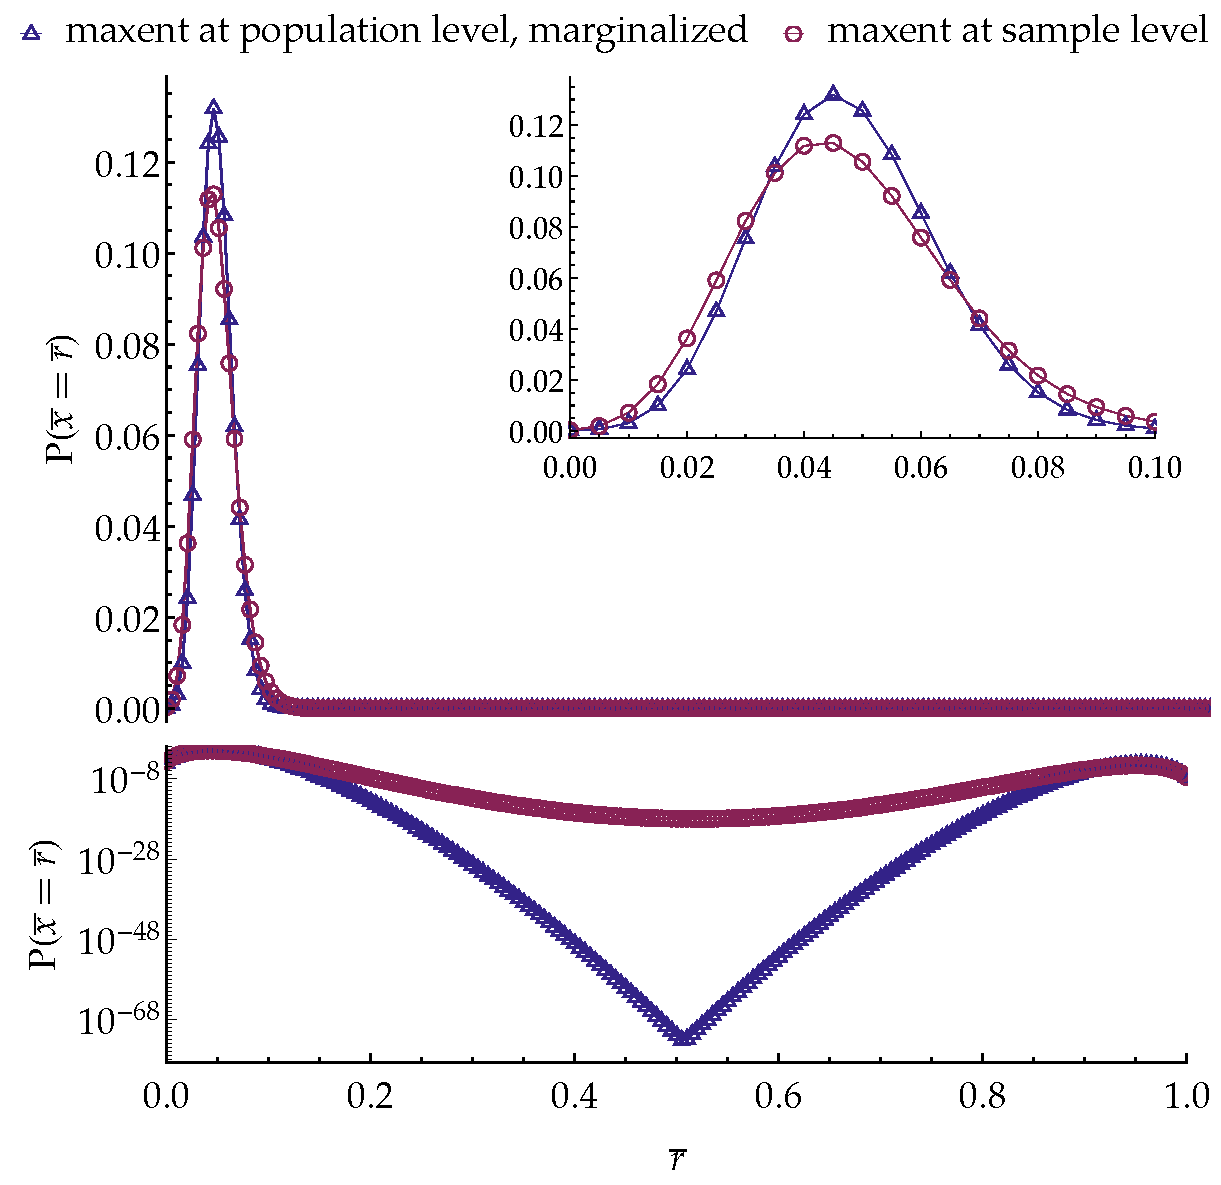
\includegraphics[width=\linewidth]{different_maxent_pop_sample_200_realdata_2mom.pdf}%
\caption{Linear and log-plots of $\pf(\ya)$ constructed by \me\ at
  the network level followed by sample marginalization (blue triangles),
  \eqn~\eqref{eq:app_maxent_pop_marg}, and at the sample level (red
  circles), \eqn~\eqref{eq:app_maxent_sample}, with $\yNv=5000$,
  $n=200$, and constraints as in \eqn~\eqref{eq:constraints}.}
\label{fig:diff_maxent_pop_sample}
\end{figure}%maxent_pop_or_sample.nb
%
\begin{figure}[!t]
\centering
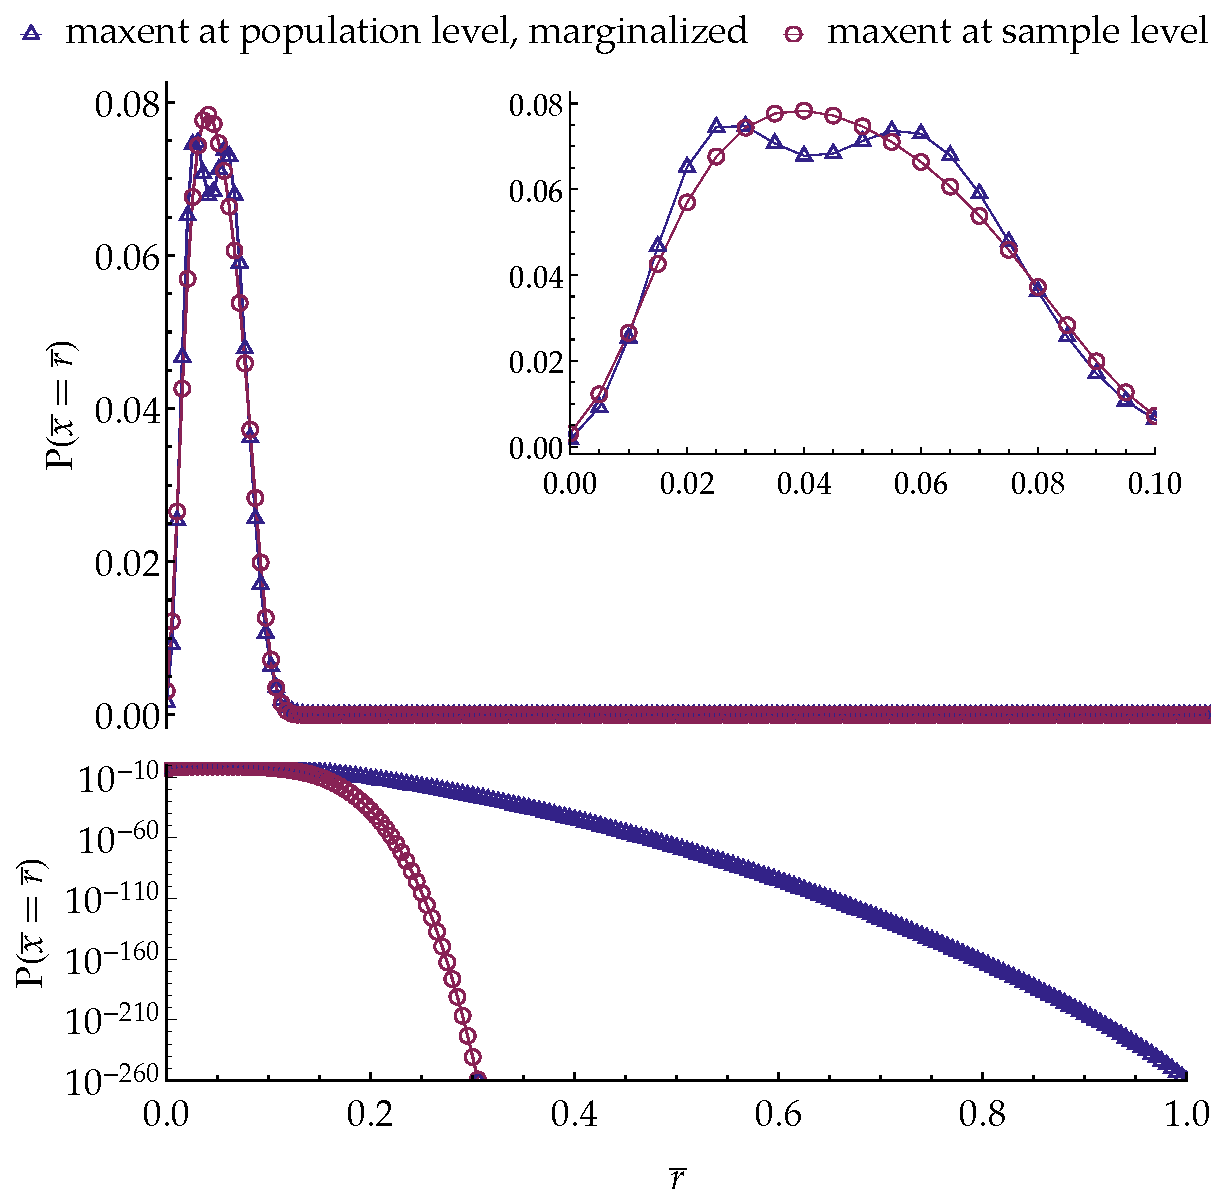
\includegraphics[width=\linewidth]{different_maxent_pop_sample_200_realdata_4mom.pdf}% 
\caption{Linear and log-plots of $\pf(\ya)$ constructed by \me\ at
  the network level followed by sample marginalization (blue triangles),
  \eqn~\eqref{eq:app_maxent_pop_marg}, and at the sample level (red
  circles), \eqn~\eqref{eq:app_maxent_sample}, with $\yNv=5000$,
  $n=200$, and constraints as in \eqn~\eqref{eq:constraints}.}
\label{fig:diff_maxent_pop_sample_realdata}
\end{figure}%maxent_pop_or_sample.nb
\fi%
\begin{figure}[!t]
\centering
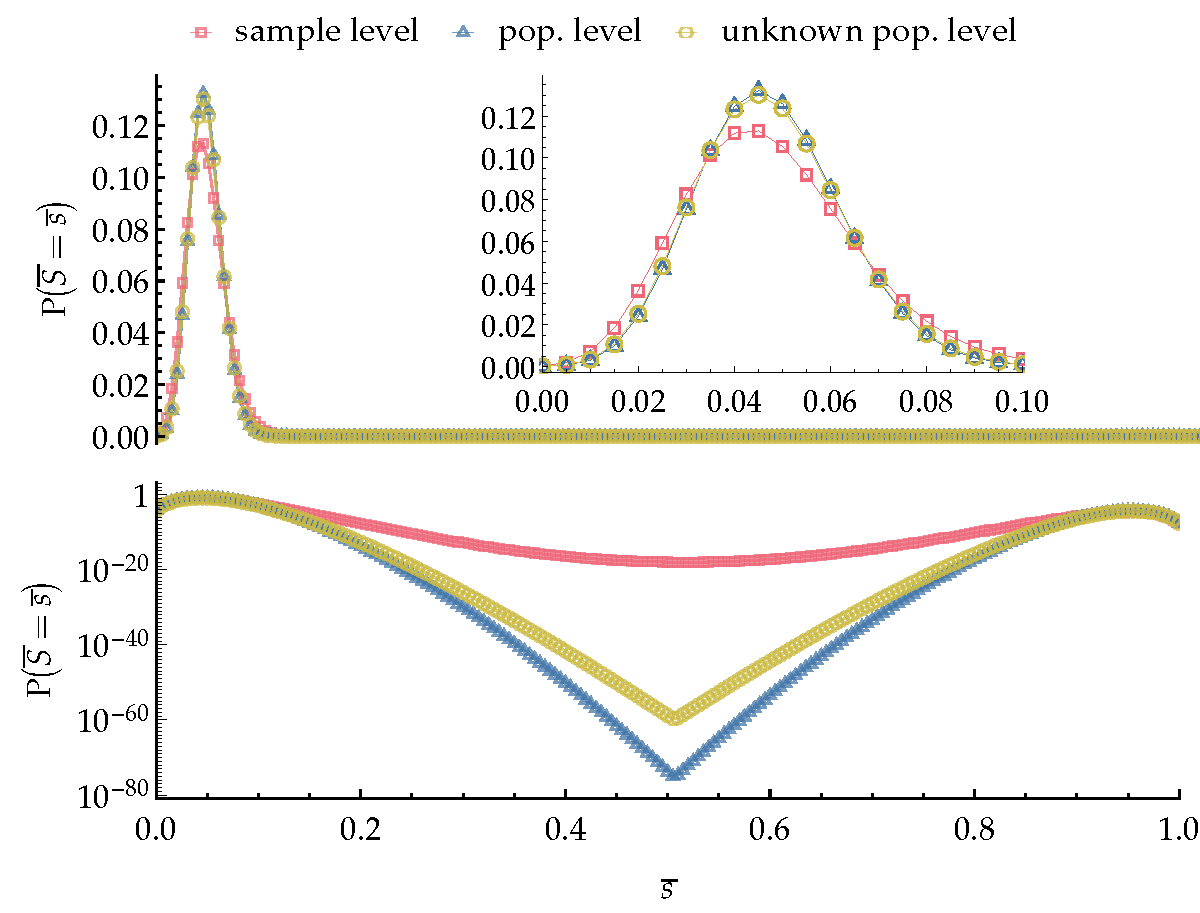
\includegraphics[width=\linewidth]{comparison3.pdf}%
\caption{Linear and log-plots of $\pf(\ya)$ for a sample of $n=200$
  and constraints as in \eqn~\eqref{eq:constraints}, constructed by:
  \textcolor{myred}{\textbf{red squares:}} \me\ at the sample level,
  \eqn~\eqref{eq:app_maxent_sample};
  \textcolor{mypurpleblue}{\textbf{blue triangles:}} \me\ at the
  network level, \eqn~\eqref{eq:app_maxent_pop_marg} with
  $\yNv=10\,000$, followed by sample marginalization;
  \textcolor{myyellow}{\textbf{yellow circles:}} \me\ at the network
  level with unknown network size,
  \eqn~\eqref{eq:app_maxent_pop_marg_unknown_N}, according to the
  distribution~\eqref{eq:pdf_popsize} for the network.}
\label{fig:all_three}
\end{figure}%maxent_pop_or_sample.nb\fi
The distribution obtained at the sample level will show different
features from the one obtained at the network level, like displaced or
additional modes or particular tail behaviour. We show an example of this
discrepancy in \fig~\ref{fig:all_three}, for
$\yNv=10\,000$, $n=200$, and the two constraints
\begin{equation}
  \label{eq:constraints}
  \E(\ya) = 0.0478,\qquad
  \E(\yaas) = 0.00257,
  % ,\quad
  % \expe{\sav{\yaa\yaa\yaa}} = 1.48\times 10^{-4},\quad
  % \expe{\sav{\yaa\yaa\yaa\yaa}} = 8.81 \times 10^{-6}.
\end{equation}
which come from the actual recording of circa 200 neurons from macaque
motor cortex \citep{rostamietal2016_r2017}. The distribution obtained at the
network level (blue triangles) has a higher and displaced mode and a quite
different behaviour for activities around $0.5$ than the distribution
obtained at the sample level (red squares).

\bigskip

In our discussion we have so far assumed the size $\yNv$ of the larger
network to be known. This is rarely the case, however. We usually are
uncertain about $\yNv$ and can only guess its order of magnitude. In such a
state of knowledge $\yHd$ our ignorance about the possible value of $\yNv$
is expressed by a probability distribution $\pf(\yNN=\yNv \|\yHd)=h(\yNv)$,
and the marginal distribution for the sample
activity~\eqref{eq:app_maxent_pop_marg} is modified, by the law of total
probability, to
\begin{multline}
  \label{eq:app_maxent_pop_marg_unknown_N}
  \pf(\ya \| \yHd)  =
  \sum_{\yNv} \pf(\ya \| \yNv,\yHd) \,
  \pf(\yNv \|\yHd)
  ={}\\[-\jot]
  \sum_\yNv \biggl\{\frac{1}{\yK(\yll_\yNv)}\, 
  \sum_{\yA} \ypp^{(\yNv)}_{\ya\yA}
\,
  \tbinom{\yNv}{\yNv \yA}\,\exp\Bigl[{\yll_\yNv}\T
  \tsum_{\ya} \yg_{\ya}\ypp^{(\yNv)}_{\ya\yA}\Bigr]\biggr\}
  \;h(\yNv),
\end{multline}
where the Lagrange multipliers $\yll_{\yNv}$ and the summation range for
$\yA$ depend on $\yNv$.

As a proof of concept, \fig~\ref{fig:all_three} also shows such a distribution
(yellow circles) for the same constraints as above, and a probability
distribution for $\yNv$ inspired by Jeffreys
\citep[\sect~4.8]{jeffreys1939_r1983}:
\begin{equation}
  \label{eq:pdf_popsize}
  h(\yNv) \propto 1/\yNv, \qquad
  \yNv \in\set{1\,000,\; 2\,000,\; \dotsc,\;10\,000}.
\end{equation}

\section{Derivation from the probability calculus}
\label{sec:derivation_prob_calculus}

There are three inequivalent main routes that lead to a probability
distribution of the maximum-entropy form~\eqref{eq:app_maxent_sample}
or~\eqref{eq:app_maxent_pop}. The distribution carries a different
interpretation under each route \citep[pp.~52--55,
72--77]{jaynes1979b}[pp.~25--28]{jaynes1982}[\sect~I]{jaynes1982b}{jaynes1986d_r1996}[\sect~11.1]{jaynes1994_r2003}.

\begin{enumerate}[wide,label=(\alph*)]
\item \label{item:entropy_route}One route is the choice of the distribution having the highest
  Shannon entropy, given only a quantitative assessment some of its
  properties, such as expectations. The numerical choice of the value of
  such properties is a (subjective) assumption.

  \medskip

  In the two other routes the maximum-entropy distribution is obtained as
  an \emph{approximation} of a distribution obtained via the probability
  calculus, using data coming from a set of $T$ measurements -- as in our
  present case.\mynote{refs here} Also in this case some (subjective)
  assumptions are necessary: they concern our beliefs about the long-run
  relative frequencies of the measurement outcomes:\footnote{Such
    assumptions are always necessary at the beginning of an inference:
    \enquote{Now the axioms of probability enable us to infer any
      probability-conclusion \emph{only} from probability-premisses. In
      other words, the calculus of probability does not enable us to infer
      any probability-value unless we have some probabilities or
      probability relations \emph{given}. Such data cannot be supplied by
      the mathematician. E.g. the rules of arithmetic and the axioms of the
      probability-calculus are utterly impotent to determine, on the
      supposed knowledge that the throw of a coin must yield either head or
      tail and cannot yield both, the probability that it will yield head
      or that it will yield tail. We must assume that the two co-exclusive
      and co-exhaustive possibilities are \emph{equally probable}, before
      we can estimate the probability of either as being a half of
      certitude} \citep[\emph{Appendix on eduction}, \sect~5,
    p.~182]{johnson1924}.}

\item \label{item:entr_prior_route}In one case we consider all possible
  sets of measurement outcomes to be \emph{roughly} equally likely; this
  leads to a probability for the frequencies $\ynu$ proportional to a
  multinomial coefficient $\binom{L}{L\ynu}$, with $L$ large but smaller
  than $T$. (We cannot assume the sets of measurement outcomes to be
  exactly equally likely, because this is equivalent to their independence:
  \cf\
  \cites[\sect~6.7]{jaynes1994_r2003}[\sect~B]{portamana2009}[\sect~2]{portamana2017}.)
  The exact expression is\mynote{equation here}
  %   \begin{multline}
  %   \label{eq:prob_conditional_average_exch}
  %   \p\bigl[\yE{N+1}{k} \bigcond \tsum\yo\yf{N}\in\yA, \yX\bigr] ={}\\
  %   \frac{\int\yqq_k\sum_{\yf{N}}  \delt(\tsum \yo\yf{N}\in \yA)\,
  %     \binom{N}{N\yf{N}}\,\bigl( \tprod \yq^{N\yf{N}} \bigr)  \,
  %     \pf(\yq \|\yX)  \,\di\yq}{ \int\sum_{\yf{N}} \delt(\tsum \yo\yf{N}\in \yA)\,
  %     \binom{N}{N\yf{N}}\,\bigl( \tprod \yq^{N\yf{N}} \bigr) \,
  %     \pf(\yq \|\yX) \,\di\yq },
  % \end{multline}

\item \label{item:suff_route}In the other case we assume that the
  measurements have a \emph{sufficient statistics}: the same as appears in
  the exponential of the maximum-entropy distribution. The exact expression is\mynote{equation here}
  % \begin{multline}
  %   \label{eq:prob_conditional_average_suff}
  %   \p\bigl[\yE{N+1}{k} \bigcond \tsum\yo\yf{N}\in\yA, \yS\bigr] ={}
  %       \\[3\jot]
  %    \frac{\int \pf(k \| \yl,\yaa,\yS) \sum_{\yf{N}} \delt(\tsum \yo\yf{N}\in \yA)\,
  %     \binom{N}{N\yf{N}}\,\bigl[ \tprod  \pf(\yk \| \yl,\yaa,\yS)^{N\yf{N}} \bigr]
  %      \,
  %     \pf(\yl \|\yS) \,\di\yl}{\int\sum_{\yf{N}} \delt(\tsum \yo\yf{N}\in \yA)\,
  %     \binom{N}{N\yf{N}}\,\bigl[ \tprod \pf(\yk \| \yl,\yaa,\yS)^{N\yf{N}} \bigr]
  %      \,
  %     \pf(\yl \|\yS) \,\di\yl}.
  % \end{multline}
\end{enumerate}

It's important to keep in mind that the approximate equivalence of these
three routes only holds under very specific assumptions -- which \emph{have
  physical and biological meanings and consequences}. In particular,
route~\ref{item:suff_route} implies that we can discard other empirical
statistics of the data, if they are known; whereas
route~\ref{item:entr_prior_route} requires us to specify all known
empirical statistics, because using only a subset of them may lead to
different results. Route~\ref{item:entropy_route} is also supposed to be
used with all known data. Moreover, the approximate equivalence of
route~\ref{item:entropy_route} with routes~\ref{item:entr_prior_route} and
\ref{item:suff_route} \emph{only holds if $T$ is much larger than the
  possible values of the activity $\yA$}. Finally, we also obtain very
different expressions depending on whether we're asking about \emph{the
  activity in one of the \textbf{recorded} time bins} or about \emph{the
  activity in a \textbf{new} time bin}. Works that use maximum-entropy
distributions are often very vague about the latter point.


\bigskip

Here are the distributions for our \dobs\ about three different quantities,
assuming an entropic pre-data distribution for the long-run frequencies of
the full network:

\textbf{The frequency distribution $\yF$ of the full-network activity
  \emph{during the recording}}

\begin{equation}
  \label{eq:fullfreq_from_samplefreq}
  \begin{split}
  \p(\yF \|\yf,\yH) &\propto
  \!\begin{multlined}[t][0.8\linewidth]
  \int\!\di\ynu\;  \tsum_{\yj}
  \delt(\tsum_{\yA}\yjj_{\ya\yA} = \yff_{\ya})\;
  \delt(\tsum_{\ya}\yjj_{\ya\yA} = \yFF_{\yA})\times{}\\
  \binom{T}{T\yj}\;
  \biggl[\prod_{\ya\yA}
(\ypp_{\ya\yA}\ynuu_{\yA})^{T\yjj_{\ya\yA}}
\biggr]\;
\exp[-L\;\ysh(\ynu;\yR)]
\end{multlined}
\\
&\appropto \delt(\tsum_{\yA}\ypp_{\ya\yA}\yFF_{\yA} = \yff_{\ya})\;
\exp[-L\;\ysh(\yF;\yR)]
\end{split}
\end{equation}

\bigskip

\textbf{The long-run frequency distribution $\ynu$ of the full-network
  activity}

\begin{equation}
  \label{eq:longrun_from_samplefreq}
  \begin{split}
  \p(\ynu \|\yf,\yH) &\propto
    \binom{T}{T\yf}\;
  \biggl[\prod_{\ya}
(\tsum_{\yA}\ypp_{\ya\yA}\ynuu_{\yA})^{T\yff_{\ya}}
\biggr]\;
\exp[-L\;\ysh(\ynu;\yR)]
\\
&\appropto 
\exp[-T\;\ysh(\yf; \mathte{\ypp}\ynu)
-L\;\ysh(\ynu;\yR)]
\end{split}
\end{equation}
Note that if some $\yff_{\ya}$ are zero, then the first exponential may
be badly approximated by a delta, because the constraints lie on a facet of the
simplex of frequencies $\set{\ynu}$.

\bigskip

\textbf{The activity $\yA'$ of the full-network
  in a \emph{new} time bin}

\begin{equation}
  \label{eq:newbin_from_samplefreq}
  \begin{split}
  \p(\yA' \|\yf,\yH) &\propto
  \int\!\di\ynu\;\ynuu_{\yA'}\;
  \binom{T}{T\yf}\;
  \biggl[\prod_{\ya}
(\tsum_{\yA}\ypp_{\ya\yA}\ynuu_{\yA})^{T\yff_{\ya}}
\biggr]\;
\exp[-L\;\ysh(\ynu;\yR)]
\\
&\appropto 
\int\!\di\ynu\;\ynuu_{\yA'}\;
\exp[-T\;\ysh(\yf; \mathte{\ypp}\ynu)
-L\;\ysh(\ynu;\yR)]
\end{split}
\end{equation}
Note that if some $\yff_{\ya}$ are zero, then the first exponential may
be badly approximated by a delta, because the constraints lie on a facet of the
simplex of frequencies $\set{\ynu}$.

\bigskip

The maximum-relative-entropy distribution is, in the first two cases, an
approximation of the most probable frequency distribution $\yF$ or $\ynu$;
in the third case, an approximation of the probability distribution for
$\yA'$.

\section{Assumptions and limitations}
\label{sec:assumptions}

Main assumptions behind this belief distribution:

We are approximating our state of knowledge with a finitely exchangeable
one. In turn, this is numerically approximated by an infinitely
exchangeable one for $T$ large. But we don't really have an exchangeable
belief: our \dob\ that the activity at the next time bin will
differ from the activity at the present one is roughly proportional to the
difference in the two subsequent activities.

The formulae say that we have equal beliefs about the underlying network
states having the same activity. This isn't really our belief, for we
believe there are interactions between the neurons and subnetworks thereof.


\section{Discussion}
\label{sec:discussion}

The purpose of the present work was to point out and show, in a simple
set-up, that the \me\ method can be applied to recorded neuronal data in a
way that accounts for the larger network from which the data are
sampled, \eqns~\eqref{eq:app_maxent_pop}--\eqref{eq:app_maxent_pop_marg}.
This application leads to results that differ from the standard application
which only considers the sample in isolation,
\eqns~\eqref{eq:app_maxent_sample}--\eqref{eq:app_maxent_sample_constraints}.
We gave a numerical example of this difference. We have also shown how to
extend the new application when the size of the larger network is
unknown, \eqn~\eqref{eq:app_maxent_pop_marg_unknown_N}.

The latter formula, in particular, shows that the standard way of applying
\me\ 
implicitly assumes that \emph{no} larger network exists beyond the
recorded sample of neurons. One could in fact object to the application at
the network level, and say that the traditional way of applying \me,
\eqn~\eqref{eq:app_maxent_sample}, yields different results because it does
not make assumptions about the size $\yNv$ of a possibly existing larger
network. Such a state of uncertainty, however, is correctly formalized
according to the laws of probability by introducing a probability
distribution for $\yNv$, and is expressed by
\eqn~\eqref{eq:app_maxent_pop_marg_unknown_N}. This expression cannot
generally be equal to~\eqref{eq:app_maxent_sample} unless the distribution
for $\yNv$ gives unit probability to $\yNv=n$; that is, unless the sample
\emph{is} the full network, and no larger network exists.

The standard \me\ approach therefore assumes that the recorded neurons
constitute a special subnetwork, isolated from the larger network of
neurons in which it is embedded, and which was also present under the
recording device. This assumption is unrealistic. The \me\ approach at the
network level does not make such assumption and is therefore preferable.
It may reveal features in a data set that were unnoticed by the standard
\me\ approach.

% This hidden assumption of isolation is unreasonable. It amounts to say that
% the neurons we distinguished and tracked with our recording device are a
% very special, isolated set among all those that could have been recorded.
% It is for this reason that we find the \me\ application at the network
% level preferable. Physical models of neuronal networks usually include some
% sort of external input, mimicking an embedding in a larger network. The
% \me\ distribution obtained at the network level may reveal features in a
% data set that were unnoticed by the standard \me\ model.


The difference in the resulting distributions between the applications at
the sample and at the network levels appears in the use of Boltzmann
machines with hidden units \citep{lerouxetal2008}, although by a different
conceptual route. It also appears in statistical mechanics: if a system is
statistically described by a \me\ Gibbs state, its subsystems cannot be
described by a Gibbs state \citep{maesetal1999}. A somewhat similar
situation also appears in the statistical description of the final state of
a non-equilibrium process starting and ending in two equilibrium states: we
can describe our knowledge about the final state either by (1) a Gibbs
distribution, calculated from the final equilibrium macrovariables, or (2)
by the distribution obtained from the Liouville evolution of the Gibbs
distribution assigned to the initial state. The two distributions differ
(even though the final \emph{physical} state is obviously exactly the same
\citep[\sect~4]{jaynes1985d_r1993}), and the second allows us to make
sharper predictions about the final physical state thanks to our knowledge
of its preceding dynamics. In this example, though, both distributions are
usually extremely sharp and practically lead to the same predictions. In
neuroscientific applications, the difference in predictions of the sample
\vs\ full-network applications can instead be very relevant.

The idea of the new application leads in fact to more questions. For
instance:
\begin{itemize}
\item Do the standard and new applications lead to different or contrasting
  conclusions about \enquote{cooperativity}, when applied to real data
  sets?
\item How to extend the new application to the \enquote{inhomogeneous} case
  \citep{schneidmanetal2006,shlensetal2006,roudietal2009b}, in which
  expectations for individual neurons or groups of neurons are constrained?
\item What is the mathematical relation between the new application and
  \me\ models with hidden neurons
  \citep{smolensky1986,kulkarnietal2007,huang2015,dunnetal2017}?
\end{itemize}
Owing to space limitations we must leave a thorough investigation of these
questions to future work.

Finally, we would like to point out the usefulness and importance of the
probability formulae that relate our states of knowledge about a network
and its samples, presented in \sect~\ref{sec:prob_samples}. This kind of
formulae is essential in neuroscience, where we try to understand
properties of extended brain areas from partial observations. The
formulae presented here reflect a simple, symmetric state of ignorance.
More work is needed \citep[\cf][]{levinaetal2017} to extend these formulae
to account for finer knowledge of the cerebral cortex and its network
properties.


\clearpage

\hrule
\newcounter{dummy}\refstepcounter{dummy}\label{orig_intro}
\mynote{orig intro}
Experimental technologies to record the activity of many neurons at the
same time in different species and brain areas are rapidly advancing. These
experimental advancements are paralleled by advances in theoretical and
computational methods for analyzing the data accumulated using the
recording technologies. Such theoretical methods usually take the form of
probabilistic models that try to describe the multi-neuronal activity of
the recorded neurons. With such probabilistic models one aims to address
numerous issues: What correlations are important in describing the
multi-neuronal pattern? How does the pattern of activity covary with
external stimuli or experimental conditions? What dimensionality does the
neural data live in and how is this related to the underlying network
interactions? The probabilistic models can also be used to make predictions
about the structure of the neural code, by studying the properties of the
fitted model, or by generating synthetic data from it.

In general, despite the rapid advances in recording technology, the best
experimental measurements of neuronal activity still only provide data from
a small subset of neurons that comprise a neuronal network. A wealth of
studies on building probabilistic models of neural data focuses on
describing such subsets, ignoring the fact that the observed neurons is a
small group in a much bigger set of hidden neurons. Some other studies do
include hidden variables which, amongst other things, aim to model the
global features of the unrecorded neurons, but we still lack a through
understanding of how to include the role of hidden neurons in probabilistic
models, how our inferences about the recorded activity would be affected by
them, and what we can we say about the rest of the network by studying the
heavily subsampled recordings. In this paper, we aim to address these
questions in the case of a simple maximum entropy model, namely the
homogeneous maximum entropy model.

The maximum entropy approach has been used in a variety of setting for
building statistical models of complex systems and datasets, ranging from
neuronal activity in the retina, in the cortex, protein sequences, gene
regulatory networks and natural images. The general idea is, for a dataset,
to write down the distribution that maximizes the entropy of state
variables, given some low order statistics. Now given the fact that the
recorded neurons are a fraction of the neurons in the network, several
quantitative questions arise that we will address in this paper: given the
data from the sampled neurons, can we build a maximum entropy model over
the whole network? Once we build such a network level maximum entropy
model, can we see features in the neural activity which cannot be directly
seen from a model build from the sampled neurons? Since we can marginalize
down the network level maximum entropy model to the sampled network, how
does this margianzlied maximum entropy model match the sample level model?

All these questions can be answered in the case of the homogeneous maximum
entropy model. First we show how to go from the sample level maximum
entropy level to the network level, by assuming different sizes of the
network and also by assuming an uninformative prior over the size of the
network. This is done by inferring the statistics of correlation functions
at the network level from those of the sample level by using simple
counting arguments. We then find that, when applied to experimental
recordings from the Medial Entorhinal Cortex of rats and the monkey visual
cortex, this network level maximum entropy model may exhibit features that
the sample level model does not predict. Specifically, we observed modes in
the distribution of the activity in the network level model that do not
show up in the sample level. We study how the assumed size of the full
network affects the appearance of these modes and find that there is a
minimum size of the full network for which such modes can be observed. We
then compared the distribution found by marginalizing the full network
maximum entropy model down to the sample level, and the distribution fit
directly to the sample level. For the two datasets that we tested, we found
that the two distributions match each other to a large degree but that
there are also differences between them. We quantify how these differences
also depend on the assumed size of the network and find that …(WE SHOULD
TEST SHI) This predicts that for a large enough network (DO WE PREDICT
THAT IF THE FULL NETWORK GETS BIGGER THE DIFFERENCE ALSO GET BIGGER)?…

The rest of the paper is organized as follows. We first describe how to go
from the sample level maximum entropy model to the full network maximum
entropy model. In section 2, we apply this to the two experimental datasets
and study the effect of the assumed size of the network as well as the
moments that we use for building the maximum entropy model. In section 3 we
compare the distributions found from marginalizing the maximum entropy
model down to the sample level and the original sample level model.


\hrule
\bigskip


%%\setlength{\intextsep}{0.5ex}% with wrapfigure
%\begin{figure}[p!]%{r}{0.4\linewidth} % with wrapfigure
%  \centering\includegraphics[trim={12ex 0 18ex 0},clip,width=\linewidth]{maxent_saddle.png}\\
%\caption{caption}\label{fig:comparison_a5}
%\end{figure}% exp_family_maxent.nb


%%%%%%%%%%%%%%%%%%%%%%%%%%%%%%%%%%%%%%%%%%%%%%%%%%%%%%%%%%%%%%%%%%%%%%%%%%%%
%%% Acknowledgements
%%%%%%%%%%%%%%%%%%%%%%%%%%%%%%%%%%%%%%%%%%%%%%%%%%%%%%%%%%%%%%%%%%%%%%%%%%%% 
\iffalse
\begin{acknowledgements}
  PGLPM thanks Mari, Miri, \amp\ Emma for continuous encouragement and
  affection; Buster Keaton and Saitama for filling life with awe and
  inspiration; the developers and maintainers of \LaTeX, Emacs, AUC\TeX,
  Open Science Framework, Python, Inkscape, Sci-Hub for making a free and
  unfiltered scientific exchange possible.
%\rotatebox{15}{P}\rotatebox{5}{I}\rotatebox{-10}{P}\rotatebox{10}{\reflectbox{P}}\rotatebox{-5}{O}.
\sourceatright{\autanet}
\end{acknowledgements}
\fi

%%%%%%%%%%%%%%%%%%%%%%%%%%%%%%%%%%%%%%%%%%%%%%%%%%%%%%%%%%%%%%%%%%%%%%%%%%%%
%%% Appendices
%%%%%%%%%%%%%%%%%%%%%%%%%%%%%%%%%%%%%%%%%%%%%%%%%%%%%%%%%%%%%%%%%%%%%%%%%%%% 
\clearpage
% %\renewcommand*{\appendixpagename}{Appendix}
% %\renewcommand*{\appendixname}{Appendix}
% %\appendixpage
% \appendix

%%%%%%%%%%%%%%%%%%%%%%%%%%%%%%%%%%%%%%%%%%%%%%%%%%%%%%%%%%%%%%%%%%%%%%%%%%%%
%%% Bibliography
%%%%%%%%%%%%%%%%%%%%%%%%%%%%%%%%%%%%%%%%%%%%%%%%%%%%%%%%%%%%%%%%%%%%%%%%%%%% 
\defbibnote{prenote}{{\footnotesize (\enquote{de $X$} is listed under D,
    \enquote{van $X$} under V, and so on, regardless of national
    conventions.)\par}}
% \defbibnote{postnote}{\par\medskip\noindent{\footnotesize% Note:
%     \arxivp \mparcp \philscip \biorxivp}}

\printbibliography[prenote=prenote%,postnote=postnote
]

\end{document}

%%%%%%%%%%%%%%%%%%%%%%%%%%%%%%%%%%%%%%%%%%%%%%%%%%%%%%%%%%%%%%%%%%%%%%%%%%%%
%%% Cut text (won't be compiled)
%%%%%%%%%%%%%%%%%%%%%%%%%%%%%%%%%%%%%%%%%%%%%%%%%%%%%%%%%%%%%%%%%%%%%%%%%%%% 

When political elections are approaching, mass media are constantly
bubbling with results and discussions of pre-election polls. Why do we
conduct pre-election polls and other kinds of survey sampling? The
simplest, intuitive answer is \enquote{because they give us an idea of what
  the final election outcomes will be}. Can this answer be made more
quantitative?

Yes. In the simplest cases, the probability calculus give us simple and
precise quantitative relations between our expectations about a network
-- of voters, for instance -- and about a sample thereof. Suppose there are
$N$ voters, $S$ of which prefer one political candidate and $N-S$ of which
prefer another. We don't know $S$ or $N-S$. Now take a sample of $n$
voters, in such a way that we can assume that every set of $n$ voters is
equally likely to be sampled. In this sample, $s$ voters prefer the first
candidate, and $n-s$ the second. The probability calculus tells us that our
expectations of $s/n$ and $S/N$ are equal:
\begin{equation}\label{eq:poll_equal_expectations}
  \E(s/n \| \yH) = \E(S/N \| \yH),
\end{equation}
where $\yH$ represents our state of knowledge in this example. A more
precise answer to our original question then is: \enquote{because we
  \emph{expect} -- in the full probabilistic sense -- to see the same
  proportion of political preferences in a sample as in the full
  network}.

The exact equality above extends to other quantities beyond the means $S/N$
and $s/n$: it holds for all normalized \emph{factorial} moments
\citep{potts1953,broca2005}[\sect~A]{portamanaetal2015}. These expectation
equalities follow from a precise relation between our \dobs\ about the
polled voters and about all voters. The relations above are powerful
because they hold no matter what the probability distribution $\pf(S\|\yH)$
may be.

\bigskip

These probabilistic properties are of outstanding importance in
neuroscience, where we try to understand the workings of brain areas that
may include tens of thousands of neurons, but we can record only few tens
or hundreds of them. Whenever we record the activity of $n$ neurons we're
effectively polling them on the activity of all $N$ neurons under the
recording device -- those that could equally likely have been sampled
instead. Suppose the recorded activities are time-binned and binarized. At
every time bin $t$, $s(t)$ out of the $n$ neurons \enquote{vote} for
activity, and $n-s(t)$ vote for silence. The probability calculus tells us
that expectation equalities such as~\eqref{eq:poll_equal_expectations} hold
for the total activity $S(t)$ of the full network of $N$ neurons that
could have been recorded. 

Expectation properties are especially important for the maximum-entropy
method, which is used for various purposes in the neuroscientific
literature. This method is typically applied constraining the equality of
expectations and empirical averages. Expectation equalities such
as~\eqref{eq:poll_equal_expectations} then have a far-reaching consequence:
\emph{from empirical statistics of the activity of a \textbf{sample} of
  neurons we can construct maximum-entropy distributions for the total
  activity of the \textbf{full network} of neurons that could have been
  sampled by the recording device}.



% In the present work we show how to use the maximum-entropy method to assign
% a probability distribution for the total activity at a new time bin of a
% network of neurons, \emph{most of which can be unrecorded}, given
% specific statistics about the activity of a recorded \emph{sample} of the
% full network. This kind of probability assignment is extremely important
% in neuroscience: we try to understand the workings of brain areas that may
% include tens of thousands of neurons, but we can record only few tens or
% hundreds of them.

% Our approach also corrects a slight misuse of the maximum-entropy method
% as sometimes appears in the literature. When this method is applied to a
% set of neurons, it implicitly assumes that the set is completely isolated
% from other neurons. We'll reveal this implicit assumption in several ways.
% The probability distribution thus constructed is therefore affected by this
% hidden assumption. We'll study in which circumstances the application of
% the method at the sample level and at the full-network level give
% similar or different probabilities.



%%% Local Variables: 
%%% mode: LaTeX
%%% TeX-PDF-mode: t
%%% TeX-master: t
%%% End: 
